	
%\documentclass[conference]{IEEEtran}
\documentclass[smallcondensed]{svjour3}
% Some very useful LaTeX packages include:
% (uncomment the ones you want to load)

% *** MISC UTILITY PACKAGES ***
%
%\usepackage{ifpdf}
% Heiko Oberdiek's ifpdf.sty is very useful if you need conditional
% compilation based on whether the output is pdf or dvi.
% usage:
% \ifpdf
%   % pdf code
% \else
%   % dvi code
% \fi
% The latest version of ifpdf.sty can be obtained from:
% http://www.ctan.org/pkg/ifpdf
% Also, note that IEEEtran.cls V1.7 and later provides a builtin
% \ifCLASSINFOpdf conditional that works the same way.
% When switching from latex to pdflatex and vice-versa, the compiler may
% have to be run twice to clear warning/error messages.

\usepackage[english]{babel}
\usepackage[usenames]{color}
\usepackage{colortbl}
\usepackage{comment}
\usepackage{epsfig}
\usepackage{array, colortbl}
\usepackage{listings}
\usepackage{epstopdf}
\usepackage{multirow}
\usepackage{rotating}
\usepackage{subfigure}
\usepackage{subfig}
\usepackage{float}
%\usepackage[obeyspaces,hyphens,spaces]{url}
\usepackage{balance}
\usepackage{fancybox}
\usepackage{scalefnt}
\usepackage[normalem]{ulem}
\usepackage[export]{adjustbox}% http://ctan.org/pkg/adjustbox
\usepackage[table,xcdraw]{xcolor}
\usepackage{babel,blindtext}
\usepackage{graphicx}
%\graphicspath{{./pdfs}{../pdfs/}}
\usepackage{cite}
\usepackage{float}

\usepackage{amsmath}

\usepackage{listings}
\usepackage{color}
\usepackage{inconsolata}
\definecolor{dkgreen}{rgb}{0,0.6,0}
\definecolor{gray}{rgb}{0.5,0.5,0.5}
\definecolor{mauve}{rgb}{0.58,0,0.82}
\definecolor{lightgray}{rgb}{.9,.9,.9}
\definecolor{darkgray}{rgb}{.4,.4,.4}
\definecolor{purple}{rgb}{0.65, 0.12, 0.82}

\lstdefinelanguage{JavaScript}{
  keywords={typeof, new, true, false, catch, function, return, null, catch, switch, var, if, in, while, do, else, case, break},
  keywordstyle=\color{blue}\bfseries,
  ndkeywords={class, export, boolean, throw, implements, import, this},
  ndkeywordstyle=\color{darkgray}\bfseries,
  identifierstyle=\color{black},
  sensitive=false,
  numbersep=1pt,
  xleftmargin=\parindent,
  comment=[l]{//},
  morecomment=[s]{/*}{*/},
  commentstyle=\color{dkgreen}\ttfamily,
  stringstyle=\color{red}\ttfamily,
  basicstyle=\ttfamily\tiny ,
  morestring=[b]',
  morestring=[b]"
}

% *** GRAPHICS RELATED PACKAGES ***
%
%\ifCLASSINFOpdf
  % \usepackage[pdftex]{graphicx}
  % declare the path(s) where your graphic files are
  %\graphicspath{{../pdfs/}{../jpeg/}}
  % and their extensions so you won't have to specify these with
  % every instance of \includegraphics
  % \DeclareGraphicsExtensions{.pdf,.jpeg,.png}
%\else
  % or other class option (dvipsone, dvipdf, if not using dvips). graphicx
  % will default to the driver specified in the system graphics.cfg if no
  % driver is specified.
  % \usepackage[dvips]{graphicx}
  % declare the path(s) where your graphic files are
  % \graphicspath{{../eps/}}
  % and their extensions so you won't have to specify these with
  % every instance of \includegraphics
  % \DeclareGraphicsExtensions{.eps}
%\fi

% *** SPECIALIZED LIST PACKAGES ***
%\usepackage{algorithmic}

% *** ALIGNMENT PACKAGES ***
%\usepackage{array}

% *** SUBFIGURE PACKAGES ***
%\ifCLASSOPTIONcompsoc
%  \usepackage[caption=false,font=normalsize,labelfont=sf,textfont=sf]{subfig}
%\else
%  \usepackage[caption=false,font=footnotesize]{subfig}
%\fi

% *** FLOAT PACKAGES ***
%
%\usepackage{fixltx2e}
%\usepackage{stfloats}

% *** PDF, URL AND HYPERLINK PACKAGES ***
\usepackage{url}
% Basically, \url{my_url_here}.

% correct bad hyphenation here

\newcommand{\ts}{\textsuperscript}
\newcommand{\ea}{{et al.}}
\newcommand{\cf}{{\textit{cf.,}}}
\newcommand{\aka}{{\textit{a.k.a.,}}}
\newcommand{\smallsection}[1]{\noindent\textbf{#1.}}
\newcommand{\eg}{{\textit{e.g.,}}}
\newcommand{\ie}{{\textit{i.e.,}}}


\hyphenation{op-tical net-works semi-conduc-tor}
\newcommand{\Foutse}[1]{\textcolor{red}{{\it [Foutse says: #1]}}}
\newcommand{\David}[1]{\textcolor{dkgreen}{{\it [David says: #1]}}}
\newcommand{\Amir}[1]{\textcolor{red}{{\it [Amir says: #1]}}}
\newcommand{\Pooya}[1]{\textcolor{red}{{\it [Pooya says: #1]}}}
\newcommand{\New}[1]{\textcolor{red}{#1}}

\newcommand{\mytitle}[1]{\textbf{#1:}}

\newcommand{\hypobox}[1]{
  \begin{center}%
        \noindent\thicklines
        \setlength{\fboxsep}{6pt}%
        \setlength{\fboxrule}{0.7pt}%
        %\cornersize{0.3}
        \fbox{
            \begin{minipage}{3.2in}%
              \textit{#1}
            \end{minipage}
        }
  \end{center}
}

\begin{document}

\title{A Large-Scale Empirical Study of Code Smells In JavaScript Projects}
\author{David Johannes        	\and
        Foutse Khomh 	\and
        Giuliano Antoniol
}

\institute{David Johannes \at
           	SWAT Lab., Polytechnique Montr\'{e}al, QC, Canada\\
           	\email{david.johannes@polymtl.ca}
            	\and
 			Foutse Khomh \at
           	SWAT Lab., Polytechnique Montr\'{e}al, QC, Canada\\
           	\email{foutse.khomh@polymtl.ca}
               \and
           Giuliano Antoniol \at
           SOCCER Lab., Polytechnique Montr\'{e}al, QC, Canada\\
           	\email{giuliano.antoniol@polymtl.ca}
}

\date{Received: date / Accepted: date}


%\author{\IEEEauthorblockN{David Johannes, Amir Saboury, Pooya Musavi, Foutse Khomh and Giulio Antoniol}
%\IEEEauthorblockA{Polytechnique Montreal, Quebec, Canada\\
%          \{david.johannes, amir.saboury, pooya.musavi, foutse.khomh, giuliano.antoniol\}@polymtl.ca}
%}
%
%% make the title area
\maketitle

% As a general rule, do not put math, special symbols or citations
% in the abstract
\begin{abstract}

JavaScript is a powerful scripting programming language that has gained a lot of attention this past decade. Initially used exclusively for client-side web development, it has evolved to become one of the most popular programming languages, with developers now using it for both client-side and server-side application development. Similar to applications written in other programming languages, JavaScript applications contain \emph{code smells}, which are \emph{poor} design choices that can negatively impact the quality of an application.
In this paper, we perform a large-scale study of %extend the work of Amir Saboury et al.~\cite{saboury2017empirical} by investigating}
JavaScript code smells in server-side {\color{blue}and client-side} applications, with the aim to understand how they impact the fault-proneness of applications, and how they are evolved by the developers of the applications. % all along the projects}.
We detect 12 types of code smells in 1,807 releases of fifteen popular JavaScript applications (\ie{} express, grunt, bower, less.js, request, jquery, vue, ramda, leaflet, hexo, chart, webpack, webtorrent, moment, and riot) and perform survival analysis, comparing the time until a fault occurrence, in files containing code smells and files without code smells.  % {\color{blue}In a different way than our predecessors, we do the survival analysis with a line grain approach (wich means considering the lines where the code smells and the potential bugs appear), and with a line grain approach including dependencies (which means considering the lines where functions, objects, variables are called). Finally,
We also examine the introduction and removal of the code smells in the applications using survival models. All our analysis are conducted at the granularity of the line of code. %, we examine the perform a survival analysis on code smells to know how long they survive.
Results show that (1) on average, files without code smells have hazard rates at least 33\% lower than files with code smells. %{\color{blue}in our line grain analysis, and 45\% lower in our line grain analysis considering dependencies.}
(2) Among the studied smells, ``Variable Re-assign", ``Assignment In Conditional statements", and ``Complex Code" smells have the highest fault hazard rates. (3) Code smells, and particularly ``Variable Re-assign", %\Foutse{to revise!}
are often introduced in the application when the files containing them are created. %born as code smells (i.e., they are contained in the files at their creation),
Moreover, they tend to remain in the applications for a long period of time; %are not enough removed from the system, and have a high chance of surviving a very long time after their introduction;
``Variable Re-assign" is also the most prevalent code smell. %proliferated code smells.}
Overall, code smells affect negatively the quality of JavaScript applications and developers should consider tracking and removing them early on before the release of applications to the public.

\end{abstract}

% no keywords

\lstset{
   language=JavaScript,
   backgroundcolor=\color{lightgray},
   extendedchars=true,
   %basicstyle=\footnotesize\ttfamily,
    basicstyle=\tiny ,
   showstringspaces=false,
   showspaces=false,
   numbers=left,
   %numberstyle=\footnotesize,
   numberstyle=\tiny,
   numbersep=9pt,
   tabsize=2,
   breaklines=true,
   showtabs=false,
   captionpos=b
}

\lstset{language=Javascript}

\section{Introduction}
\begin{quote}
\emph{``Any application that can be written in JavaScript, will eventually be written in JavaScript."} \newline --- Jeff Atwood ---
\end{quote}

JavaScript is a highly dynamic scripting programming language that is becoming one of the most important programming languages in the world. Recent surveys by Stack Overflow~\cite{so:survay2016} show JavaScript topping the rankings of popular programming languages for four years in a row. Many developers and companies are adopting JavaScript related technologies in production and it is the language with the largest number of active repositories and pushes on Github~\cite{githut}. JavaScript is dynamic, weakly-typed, and has first-class functions. It is a class-free, object-oriented programming language that uses prototypal inheritance instead of classical inheritance. Objects in JavaScript inherits properties from other objects directly and all these inherited properties can be changed at run-time~\cite{fard2013jsnose}. This trait can make JavaScript programs hard to maintain. Moreover, JavaScript being an interpreted language, developers are not equipped with a compiler that can help them spot erroneous and unoptimized code. As a consequence of all these characteristics, JavaScript applications often contain code smells~\cite{fowler1997refactoring}, \ie{} poor solutions to recurring design or implementation problems. However, despite the popularity of JavaScript, very few studies have investigated code smells in JavaScript applications, and to the best of our knowledge, there is no work that examines the impact of code smells on the fault-proneness of JavaScript applications. This paper aims to fill this gap in the literature. Specifically, we detect 12 types of code smells in 1,807 releases of fifteen popular JavaScript applications (\ie{} express, grunt, bower, less.js, request, jquery, vue, ramda, leaflet, hexo, chart, webpack, webtorrent, moment, and riot) and perform survival analysis, comparing the time until a fault occurrence, in files containing code smells and files without code smells. Similar to our previous work Saboury et al.~\cite{saboury2017empirical}, we conduct a survival analysis of code smells in these JavaScript applications, but at the granularity of the line, \ie{} considering the lines of code where the code smells and the faults appeared. We also conduct a survival analysis of code smells aiming at understanding how long they survive in applications. We answer the following three research questions:

\textbf{(RQ1) Is the risk of fault higher in files with code smells in comparison with those without code smell?}
Previous works~\cite{Khomh2012,jaafar2013mining} have found that code smells increase the risk of faults in Java classes. In this research question, we compare the time until a fault occurrence in a JavaScript file that contain code smells and JavaScript files that do not contain a code smell, computing their respective hazard rates. {\color{blue} This research question replicates our previous work (\ie{}~\cite{saboury2017empirical}) but at the granularity of the line of code. In fact, in~\cite{saboury2017empirical} we analyzed the risk of fault by considering fault occurrences everywhere in a JavaScript file, \ie{} without verifying that the fault occurred on the lines of code affected by the code smells. However, a precise matching of faulty and smelly code lines is important if we want to understand the possibility of reducing the risk of fault by refactoring code smells; which is why we ensure a matching between faulty and smelly code lines in this research question (we refer to this analysis as \emph{line grain}). We also examined code lines (possibly contained in other JavaScript files) that need to be modified in order to fix the fault. For example if faulty code lines include the use or the declaration of a code element (which means an object, a function, or a variable), we add in the faulty lines the portion of code where this element is declared and used. We refer to this other analysis as \emph{line grain analysis considering dependencies}. %Specifically, we compare the time until a fault occurrence in a JavaScript file that contain code smells (and where the faulty code lines intersect with the smelly code lines, and JavaScript files without code smells (or containing code smells not affected by the fault, \ie{} there is no match between faulty and smelly code lines)}.
Results show that on average, across our fifteen studied applications, JavaScript files without code smells have hazard rates 33\% lower than files with code smells in our line grain analysis, and 45\% lower in our line grain analysis considering dependencies. These results are consistent with the findings of Saboury et al.~\cite{saboury2017empirical}}.

\textbf{(RQ2) Are JavaScript files with code smells equally fault-prone?}
A major concern of developers interested in improving the design of their application is the prioritization of code and design issues that should be fixed, considering their limited resources. This research question examines faults in files affected by different types of code smells {\color{blue}(with at least one match between faulty lines and smelly lines of the corresponding type of smell)}, with the aim of identifying code smells that developers should refactor in priority. We conduct our analysis at the granularity of the line of code as in \textbf{RQ1}. %do this research through our line grain, and line grain including dependencies analysis.}
Results show that ``Variable Re-assign", ``Assignment in Conditional Statements", and ``Complex Code" smells are consistently associated with high hazard rates across the fifteen studied systems. Developers should consider removing these code smells, in priority since they make the code more prone to faults.

\textbf{(RQ3) How long do code smells survive in JavaScript projects?}
It is interesting to know how long the smells of a project survive, when they are introduced (at the creation of a file or during a revision), and what type smell are likely to live longer. Indeed, having a good knowledge of the lifetime of code smells in JavaScript projects can help developers identify the most dangerous smell types. Our findings suggest that JavaScript code smells are often created at the file birthdate and remain in systems for a long period of time. In fact, a considerable proportion of the studied code smells still survive today in the analyzed systems. They have a high chance to survive for a very long time after their introduction into the code base. Especially, ``Variable Re-assign" which has been found to be fault-prone has one of the highest probability of surviving over time. Hence, we strongly recommend that developers remove this code smell, as soon as possible, from their projects. %at least to reduce their number.

{\color{blue}\textbf{This paper is an extension of our previous work Saboury et al.~\cite{saboury2017empirical}.} As for this previous work, we conduct a survival analysis of code smells in JavaScript applications to answer (RQ1) and (RQ2). Unlike this previous work, which made these survival analysis at the granularity of the file and on five large Javascript applications, we make our analysis at the granularity of the line of code. We also added ten more Javascript applications to our analysis. Our line grain analysis is used to refine the conclusions of this previous work : in fact, if a file is smelly and faulty, we intersect the faulty lines and the smelly lines of the file to see if a match occurs; if there is no match between faulty and smelly lines, the match obtained by Saboury et al.~\cite{saboury2017empirical} at the file level is removed from our analysis. Additionally, we examine the evolution of the studied code smells (from their introduction in the code to their last occurrence in the code) to understand how they are currently being evolved and maintained in JavaScript projects (RQ3).}

\textbf{The remainder of this paper is organized as follows.} Section \ref{sec:background} describes the type of code smells we used in our study.
Section~\ref{setup} describes the design of our case study. Section \ref{sec:case-study} presents and discusses the results of our case study. Section~\ref{threats} discusses the limitation of our study. Section \ref{sec:related} discusses related works on code smells and JavaScript systems, while Section~\ref{conclusion} concludes the paper.

\section{Background}\label{sec:background}

To study the impact of code smells on the fault-proneness of server-side JavaScript applications, and to study the smells's survival, we first need to identify a list of JavaScript bad practices as our set of code smells. Hence, we select 12 popular code smells from different JavaScript Style Guides~\cite{fard2013jsnose, npmjss, nodejss, airbnbjss, jqueryjss, ESLint}. {\color{blue}These smells are popular because, according to~\cite{fard2013jsnose, npmjss, nodejss, airbnbjss, jqueryjss, ESLint}, they widely appear in JavaScript codes, make the code unreadable, and are an obstacle to a good development of JavaScript projects.} %These smells were pre, which are the same as those studied in~\cite{saboury2017empirical}.
These code smells are presented in details in~\cite{saboury2017empirical}, {\color{blue} with their frequency of occurrences in popular JavaScript projects like JQuery} :
\begin{itemize}
	\item \textbf{Lengthy Lines} appear when there are too many characters in a single line of code.
	\item \textbf{Chained Methods} appear when there is a ``chain'' of method calls (repeated chaining method). Chaining method is a common practice in object-oriented programming languages, that consists in using an object returned from one method invocation to make another method invocation.
	\item \textbf{Long Parameter List} happens when a function has too many parameters.
	\item \textbf{Nested Callbacks} are introduced in the code when multiple asynchronous tasks are invoked in sequence (\ie{} the result of a previous one is needed to execute the next one)~\cite{brodu2015toward, gallaba2015don}.
	\item \textbf{Variable Re-assign} corresponds to the reuse of variables in the same scope for different purposes.
	\item \textbf{Assignment in Conditional Statements} occurs when the \texttt{=} operator is used in conditions. For example: $if ( a = b )$
	\item \textbf{Complex Code} smell appears when a JavaScript file is characterized by high cyclomatic complexity values (\ie{} high numbers of linearly independent paths through the code~\cite{mccabe1976complexity}).
	\item \textbf{Extra Bind} occurs most of time when we let ``\texttt{.bind(ctx)}'' on a function after removing a \texttt{this} variable from the body of the inner function, which is an unnecessary overhead.
	\item \textbf{This Assign} happens specifically when a \texttt{this} variable is stored in another variable to access to the parent scope's context.
	\item \textbf{Long Methods} is a well-known code smell \cite{marinescu2006object, fard2013jsnose, fontana2012automatic} which consists in writing a method with too many statements.
	\item \textbf{Complex Switch Case} happens when there are too many switch statements.
	\item \textbf{Depth} smell occurs when the number of nested blocks of code (or the level of indentation) is too high.
\end{itemize}
{\color{blue}Table~\ref{smellscount} indicates the number of smells, by type, that we found in each studied JavaScript project (including all their commits). We can notice that all the studied JavaScript projects, even those proposing a Style Guide to avoid code smells (like JQuery), contain a large number of code smells. Plus, each type of code smell is highly diffused in at least one studied JavaScript project.}
%For more clarifications about the twelve studied code smells, please look at the work of Amir Saboury et al.~\cite{saboury2017empirical}, section II.}

\begin{table*}[!htbp]
{\color{blue}
\centering
\footnotesize
\caption{{\color{blue}Smells count of the studied systems.}}
\label{smellscount}
\resizebox{1.3\linewidth}{!}{
\begin{tabular}{l|l|l|l|l|l|l|l|l|l|l|l|l|l}
\hline
\textbf{Module}  & \textbf{Long} & \textbf{Depth} & \textbf{Complex} & \textbf{Lengthy} & \textbf{Long} & \textbf{Nested} & \textbf{Complex} & \textbf{Chained} & \textbf{Variable} & \textbf{Extra} & \textbf{Assignment in}& \textbf{This} & \textbf{Total} \\
& \textbf{Methods} & & \textbf{Code} & \textbf{Lines} & \textbf{Parameter} & \textbf{Callbacks} & \textbf{Switch} & \textbf{Methods} & \textbf{Re-assign} & \textbf{Bind} & \textbf{Conditional}& \textbf{Assign} & \\
& & & & & \textbf{List} & & \textbf{Case} & & & & \textbf{Statements}& & \\ \hline
Express       & 3313 & 104  & 5507 & 51802 & 2737 & 25834 & 949 & 28287 & 73116 & 0   & 1159 & 3034 & 195842 \\ \hline
Request       & 4682  & 0    & 8006  & 69496 & 374  & 1146  & 625 & 17595 & 119215 & 0   & 0   & 7214  & 228353  \\ \hline
Less.js       & 17086 & 1799  & 46940 & 361171 & 11082 & 868  & 4819 & 55608 & 482752 & 0   & 22655 & 4075 & 1008855 \\ \hline
Bower.io      & 1919  & 0    & 3017  & 101901 & 356  & 25687 & 8   & 143999 & 72712 & 123 & 0   & 2145  & 351867 \\ \hline
Grunt         & 1393  & 28    & 1901  & 54269 & 433  & 1039  & 10   & 17931 & 29734 & 3   & 113 & 22    & 106876  \\ \hline
Jquery	      & 39002 & 3389 & 45664 & 1197334 & 12397 & 14036 & 897 & 409512 & 518637 & 3   & 811 & 3913 & 2245595 \\ \hline
Vue.js        & 25009  & 1509  & 64842  & 230084  & 21458  & 159   & 259  & 7338  & 462302  & 0   & 1201 & 9780  & 823941  \\ \hline
Ramda 	      & 1754  & 9    & 3855  & 427837 & 5237  & 3013 & 974 & 10700 & 158314 & 0   & 5   & 526  & 612224 \\ \hline
Leaflet	      & 7382 & 0    & 32934 & 263223 & 7648 & 10249  & 2800 & 138734 & 357790 & 0   & 733 & 244  & 821737 \\ \hline
Hexo.io	      & 2023 & 45   & 4626 & 34250 & 1433  & 12263 & 580 & 71734 & 57196 & 0   & 243  & 1100  & 185493 \\ \hline
Chart.js      & 14776 & 22    & 33706 & 457036 & 7643 & 4720  & 2795 & 357635 & 409079 & 0   & 2005 & 13961 & 1303378 \\ \hline
Webpack	      & 4337 & 176   & 7354 & 122926 & 2869 & 9806 & 2249 & 66051 & 77397 & 69  & 28  & 608  & 293870 \\ \hline
Webtorrent.io & 18956  & 1059   & 48636  & 42989 & 11913  & 3437  & 2449 & 418806 & 653364 & 0   & 631 & 44645  & 1246885  \\ \hline
Moment	      & 23927 & 107   & 47334 & 1177712 & 10530 & 4743   & 6263 & 551804 & 453806 & 0   & 422  & 1064  & 2277712 \\ \hline
Riot	      & 13412 & 795  & 34536 & 209389 & 11209 & 2732  & 4301 & 28250 & 357150 & 91  & 7028 & 5652  & 674545 \\ \hline
\end{tabular}
}
\vspace{-15pt}
}
\end{table*}

\section{Study Design}\label{setup}

\begin{table*}[!htbp]
\centering
\footnotesize
\caption{Descriptive statistics of the studied systems.}
\label{studiedsystems}
\resizebox{1.3\linewidth}{!}{
\begin{tabular}{l|l|l|l|l|l|l|l|l}
\hline
\textbf{Module}   & \textbf{Domain}              		& \textbf{\# Commits} & \textbf{\# Contributors} & \textbf{\# Github stars} & \textbf{\# Releases} & \textbf{\# Closed issues} & \textbf{\# Forks} & \textbf{Project start date}     \\ \hline
Express  & Web framework       		& 5500+      & 220             & 41500+          & 277         & 2800+            & 7100+    & Jun 26, 2009       	   \\ \hline
Request  & HTTP client utility 		& 2200+      & 285             & 21300+          & 144         & 1700+            & 2500+	 & Jan 23, 2011           \\ \hline
Less.js  & CSS pre-processor   		& 2800+      & 217             & 15800+          & 74          & 2300+			  & 3400+	 & Feb 20, 2010           \\ \hline
Bower.io	 & Package manager     		& 2700+      & 210             & 15200+          & 105         & 1600+ 		      & 1900+ 	 & Sep 7, 2012            \\ \hline
Grunt    & Task Runner         		& 1400+      & 67              & 11900+          & 13          & 1000+ 			  & 1500+ 	 & Sep 21, 2011           \\ \hline
Jquery	 & JavaScript library  		& 6300+		 & 273			   & 50500+			 & 148		   & 1700+			  & 17000+	 & Apr 3, 2009			   \\ \hline
Vue.js   & JavaScript framework		& 2700+		 & 240			   & 122300+			 & 233		   & 7100+			  & 17000+	 & Jul 29, 2013		   \\ \hline
Ramda 	 & JavaScript library		& 2700+		 & 212			   & 14800+			 & 49		   & 1100+			  & 900+	 & Jun 21, 2013		   \\ \hline
Leaflet	 & JavaScript library		& 6600+		 & 590			   & 23500+			 & 41 		   & 3500+			  & 3900+	 & Sep 22, 2010		   \\ \hline
Hexo.io	 & Blog framework			& 2600+		 & 125			   & 24500+			 & 130		   & 2700+			  & 3300+	 & Sep 23, 2012		   \\ \hline
Chart.js	 & JavaScript charting		& 2600+ 	 & 287			   & 40800+			 & 41		   & 3900+			  & 9200+	 & Mar 17, 2013		   \\ \hline
Webpack	 & JavaScript bundler		& 7400+		 & 500			   & 45800+			 & 331 		   & 5500+			  & 5800+	 & Mar 10, 2012 		   \\ \hline
Webtorrent.io & Streaming torrent client & 2300+	 & 116			   & 18200+			 & 277		   & 1000+			  & 1700+	 & Oct 15, 2013		   \\ \hline
Moment	 & JavaScript date manager  & 3600+		 & 480			   & 39500+			 & 74		   & 2900+			  & 5900+ 	 & Mar 1, 2011			   \\ \hline
Riot	 & Component-based UI library & 3200+ 	 & 169			   & 13300+			 & 122 		   & 1800+			  & 1000+	 & Sep 27, 2013		   \\ \hline
\end{tabular}
}
\vspace{-15pt}
\end{table*}

The \emph{goal} of our study is to investigate the relation between the occurrence of code smells in JavaScript files and the fault-proneness of the part of the JavaScript files containing the smelly code lines. We also aim to understand the survival of code smells during the evolution of the projects. The \emph{quality focus} is the source code fault-proneness, which, if high, can have a negative impact on the cost of maintenance and evolution of the system. The \emph{perspective} is that of researchers, interested in the relation between code smells and the quality of JavaScript systems. The results of this study are also of interest for developers performing maintenance and evolution activities on JavaScript systems since they need to take into account and forecast their effort, and to testers, who need to know which files should be tested in priority. Finally, the results of this study can be of interest to managers and quality assurance teams, who could use code smell detection techniques to assess the fault-proneness of in-house or to-be-acquired systems, to better quantify the cost-of-ownership of these systems. The \emph{context} of this study consists of 12 types of code smells identified in fifteen JavaScript systems. In the following, we introduce our research questions, describe the studied systems, and present our data extraction approach. Furthermore, we describe our model construction and model analysis approaches.

\textbf{(RQ1) Is the risk of fault higher in files with code smells in comparison with those without code smell?}
Prior works show that code smells increase the fault-proneness of Java classes~\cite{Khomh2012,jaafar2013mining}. Since JavaScript code smells are different from the code smells investigated in these previous studies on Java systems, we are interested in examining the impact that JavaScript code smells can have on the fault-proneness of JavaScript applications. In our previous work~\cite{saboury2017empirical} we showed that JavaScript files with code smells are more likely to be fault-proneness than those without code smells. In this research question, we will refute or confirm this conclusion by replicating the analysis at the granularity of code lines. An analysis at the granularity of code lines is important to verify if the faults observed in files containing code smells occur on the portion of code affected by the code smell(s). {\color{blue}Indeed, in our previous work, when a file is marked as smelly and faulty, there is no guarantee that the fault occurred on the part of the file containing the code smell. %  correlation between both events is made ; however, 
It is possible that the faulty code lines are different from the smelly code lines. Our current analysis at the granularity of the line do not consider this to be a match and hence refines the link between the smelliness and the fault-proneness of JavaScript files. By performing a line grain analysis, we expect the observed impact of code smells on fault-proneness to be more accurate.} %files could be minimized, but still relevant and more accurate.}
%analysing approaches with finer grain, which means a line grain approach and a line grain including dependencies approach.}

\textbf{(RQ2) Are JavaScript files with code smells equally fault-prone?}
During maintenance and quality assurance activities, developers are interested in identifying parts of the code that should be tested and--or refactored in priority. Hence, we are interested in identifying code smells that have the most negative impact on JavaScript systems, \ie{} making JavaScript applications more prone to faults.

\textbf{(RQ3) How long do code smells survive in JavaScript projects?}
We are interested here in knowing the genealogy of code smells in JavaScript projects. {\color{blue}Behind this, we aim to understand when smells are introduced (\ie{} at the birthday of files, or during changes), how long they survive, and when they are generally removed (\ie{} at the deletion of files, or through refactorings).}
%in order to understand how they are introduced, how long they survive, if they are persistent, and how they are removed (\ie{} if it happens when files are deleted or through refactorings). % they are created, and how long they last. %hw during the process life of files, and which are the most dangerous.}

\subsection{Studied Systems}
In order to address our research questions, we perform a case study with the following fifteen open source JavaScript projects. Table~\ref{studiedsystems} summarizes the characteristics of our subject systems.\\
\textbf{Express}\footnote{https://github.com/expressjs/express} is a minimalist web framework for Nodejs. It is one of the most popular libraries in NPM \cite{mardan2014express} and it is used in production by IBM, Uber and many other companies\footnote{https://expressjs.com/en/resources/companies-using-express.html}. Its Github repository has over 5,500 commits and more than 220 contributors. It has been forked 7,100 times and starred more than 41,500 times. Express is also one of the most dependent upon libraries on NPM with over 8,800 dependents. There are more than 2,800 closed Github issues on their repository.\\
\textbf{Bower.io}\footnote{https://github.com/bower/bower} is a package manager for client-side libraries.
It is a command line tool which was originally released as part of Twitter's open source effort\footnote{https://engineering.twitter.com/opensource} in 2012 \cite{bowerabout}. Its Github repository has more than 2,700 commits from more than 210 contributors. Bower has been starred over 15,200 times on Github and has over 1,600 closed issues.\\ 
\textbf{LessJs}\footnote{https://github.com/less/less.js} is a CSS\footnote{Cascading Style Sheet} pre-processor. It extends CSS and adds dynamic functionalities to it. There are more than 2,800 commits by over 210 contributors on its Github repository. LessJs's repository has more than 2,300 closed issues and it is starred more than 15,800 times and forked over 3,400 times.\\ 
\textbf{Request}\footnote{https://github.com/request/request} is a fully-featured library to make HTTP calls. More than 8,300 other libraries are direct dependents of Request. Over 2,100 commits by more than 270 contributors have been made into its Github repository and 16,000+ users starred it. There are more than 1,200 closed issues on its Github repository.\\ 
\textbf{Grunt}\footnote{https://github.com/gruntjs/grunt} is one of the most popular JavaScript task runners. More than 1,600 other libraries on NPM are direct dependents of Grunt. Grunt is being used by many companies such as Adobe, Mozilla, Walmart and Microsoft~\cite{gruntusers}. The Github repository of Grunt is starred by more than 11,900 users. More than 60 contributors made over 1,400 commits into this project. They also managed to have more than 1,000 closed issues on their github repository. We selected these projects because they are among the most popular NPM libraries, in terms of the number of installs. They have a large size and possess a Github repository with issue tracker and wiki. They are also widely used in production.\\
\textbf{JQuery}\footnote{https://github.com/jquery/jquery} is a famous JavaScript library, created to make easier the writing of client-side scripts in the HTML of web pages. It makes also easier the way to write Ajax (asynchronous JavaScript and XML) code. More than 6,300 commits have been made into its Github repository by over 270 contributors, and 50,500+ users starred it. Plus, it is forked more than 17,000 times, and there are more than 1,700 closed issues. JQuery is likely one of the most popular and biggest JavaScript project.\\
\textbf{VueJs}\footnote{https://github.com/vuejs/vue} is a performant and progressive JavaScript framework for building user interfaces. It has the big advantage (in comparison with other JavaScript frameworks) to be incrementally adoptable. Over 240 contributors made over 2,700 commits into its Github repository, and they closed more than 7,100 issues. It is forked more than 17,000 times and starred more than 122,300 times, which makes it so popular.\\
\textbf{Ramda}\footnote{https://github.com/ramda/ramda} is a functional library, which makes easier the creation of functional pipelines and functions (as sequences for example), and doesn't mutate user data. It is starred more than 14,800 times, and 212 contributors made over 2,700 commits into its Github repository.\\
\textbf{Leaflet}\footnote{https://github.com/Leaflet/Leaflet} is used for mobile-friendly interactive maps, and is designed in order to be simple, efficient, easily extended (with plugins), easy to use, and usable across desktop and mobile platforms. Its Github repository is starred by more than 23,500 users and forked by over 3,900 users. More than 590 people contribute to over 6,600 commits, and managed to have more than 3,500 closed issues on their github repository.\\
\textbf{Hexo.io}\footnote{https://github.com/hexojs/hexo} is a very fast, powerful, and simple framework designed for blog's creation. It has 125 contributors, who made more than 2,600 commits, and closed over 2,700 issues. Its Github repository is forked over 3,300 times and starred over 24,500 times.\\
\textbf{ChartJs}\footnote{https://github.com/chartjs/Chart.js} is a flexible and very simple HTML5 charting that offers to designers and developers the chance to see their data in 8 different ways, possibly scalable, customisable and animated. Its Github repository joins over 280 contributors, who closed more than 3,900 issues in over 2,600 commits. Plus, more than 9,200 users forked it and over 40,800 users starred it.\\
\textbf{Webpack}\footnote{https://github.com/webpack/webpack} is a module blunder designed for modern applications. It allows the browser to load only a few number of bundles as small as possible. Those bundles correspond to the packaged modules that the application needs. Webpack is easy to configure and to take in hand. Its Github repository has over 7,400 commits and more than 500 contributors, who closed more than 5,500 issues. It has been forked 5,800 times and starred more than 45,800 times.\\
\textbf{Webtorrent.io}\footnote{https://github.com/webtorrent/webtorrent} is a streaming torrent client especially designed for the desktop and the web browser. Almost 120 contributors made over 2,300 commits and helped to solve and close more than 1000 issues on its Github repository. It is starred more than 18,200 times.\\
\textbf{Moment}\footnote{https://github.com/moment/moment} allows users to do whatever they want with dates and times in JavaScript (which means manipulate, parse, validate, display, etc.) in a very easy way. Its Github repository has more than 3,600 commits, over 480 contributors, and more than 2,900 closed issues. It is forked more than 5,900 times and starred more than 39,500 times.\\
\textbf{Riot}\footnote{https://github.com/riot/riot} is a simple, minimalistic, and elegant component-based UI library that offers to users the necessary building blocks for modern client-side applications, some custom tags, and an elegant syntax and API. Almost 170 people contributed to its Github repository, and made more than 3,200 commits, and closed more than 1,800 issues. It is starred more than 13,300 times.

{\color{blue}The criteria of selection, for the studied systems, are based on projects' popularity and activity. Indeed, in order to make our study relevant, we need popular projects to analyse, which is indicated by the Github stars of the projects. In our case, all the studied systems have more than 5000 Github stars, which make them widely used and diffused in JavaScript community. Also, as we want our analysis and conclusions pertinent, we need active systems, that evolve a lot and all the time. This is mainly shown first by the number of commits recorded by each project, which exceed 1000 for all the studied systems ; and second by their actual activity, because commits are recently pushed on each proposed system.}
%}

%extraction.tex essentialy is a part of setup.tex

\subsection{Data Extraction}\label{extraction}
To answer our research questions, we need to mine the repositories of our fifteen selected systems. {\color{blue} Given a system, for each commit we extract information about the \emph{smelliness} of each file, identifying if the file contains code smells and the location of the smelly lines}. In addition, we need to know for each commit, if the commit introduces a bug, fixes a bug, or just modifies the file in a way that a code smell is removed or added. {\color{blue}Plus, fault-proneness lines of files related to bugs need to be extracted in order to correlate them with the extracted smelly lines of the file, if they exist.} Figure~\ref{process} provides an overview of our approach to answer RQ1 and RQ2, and Figure~\ref{process3} presents an overview of the approach followed to answer RQ3. We describe each step in our data extraction approaches below. We have implemented all the steps of our approaches into a framework available on Github\footnote{\url{https://github.com/DavidJohannesWall/smells_project}}.

\begin{figure*}[t]
\captionsetup{font=small}
\centering%
	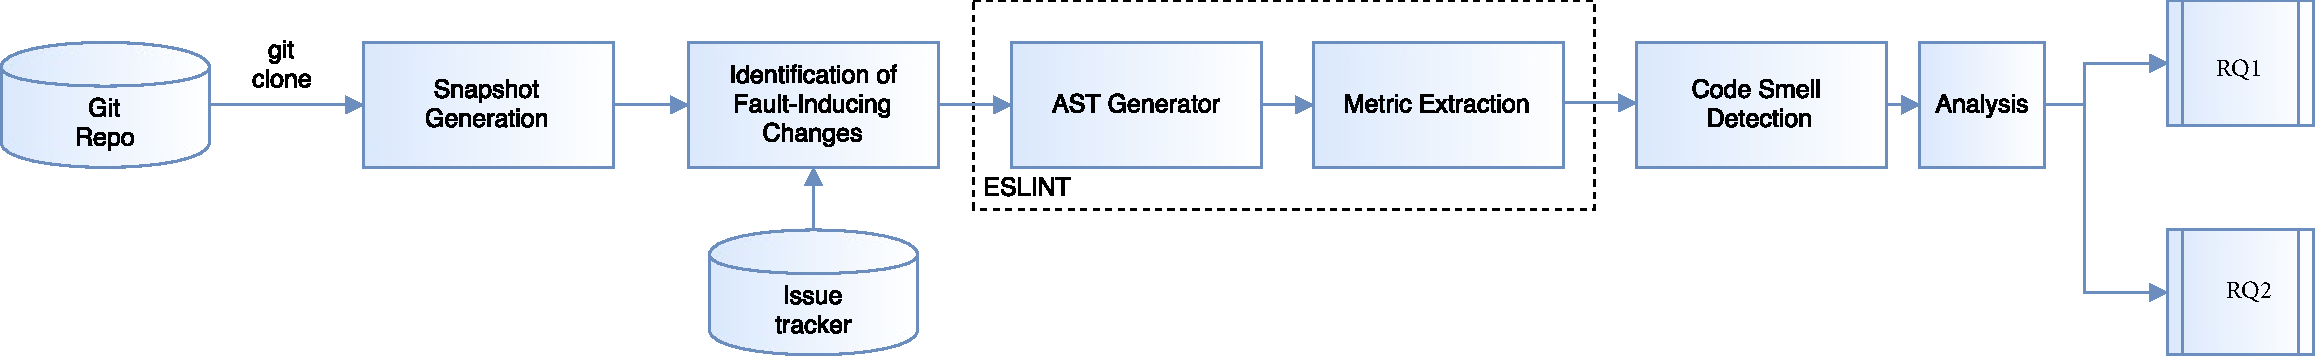
\includegraphics[scale=0.4]{total.pdf}
	\caption{Overview of our approach to answer RQ1 and RQ2.}
\label{process}
\vspace{-15pt}
\end{figure*}

\begin{figure*}[th]
	\captionsetup{font=small}
	\centering%
	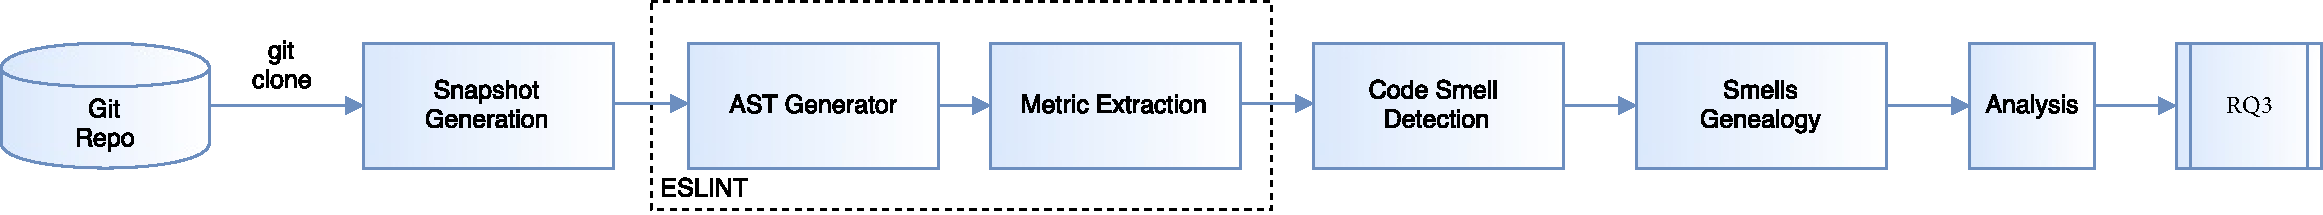
\includegraphics[scale=0.4]{total3.pdf}
	\caption{Overview of our approach to answer RQ3.}
	\label{process3}
	\vspace{-15pt}
\end{figure*}

\mytitle{Snapshot Generation} Since all the fifteen studied systems are hosted on Github, at the first step, the framework performs a \texttt{git clone} to get a copy of a system's repository locally. It then generates the list of all the commits and uses it to create snapshots of the system that would be used to perform analysis at commits level.

\mytitle{Identification of Fault-Inducing Changes} Our studied systems use Github as their issue tracker and we use Github APIs to get the list of all the resolved issues on the systems. We leverage the SZZ algorithm~\cite{sliwerski2005changes} to detect changes that introduced faults. We first identify fault-fixing commits using the heuristic proposed by Fischer et al.~\cite{fischer2003populating}, which consists in using regular expressions to detect bug IDs from the studied commit messages. {\color{blue}The regular expressions are used first to detect the information that refers to a number associated to a fixed bug ID (preceded generally by a ``\#" or a ``gh-"), and then to identify common words related to an issue fixing (\eg{} the word ``fix"). To assess the effectiveness of this heuristic, we randomly selected 100 identified fault-fixing commits from the JQuery project and examined them manually. All the 100 commits were indeed fault-fixing commits. % that introduce fault-fixing, and observe that our heuristic detect all of them. 
This result is not impressive since the best way for developers to refer to an issue, when they fix it in a commit they push on Github, is by using ``\#" or ``gh-", followed by the bug ID. In that way, especially for active projects like the studied ones, it is easy to retrieve the fault-fixing commits. However, it is possible to miss some other fault-fixing changes, either because the developers did not refer to the associated issue, or because they did it in a non common way (for example by referring to an issue number without preceding it by ``\#" or ``gh-"), or because the corresponding bug has no number ID (for these ones, this is generally because the bug is not relevant). For the JQuery project, some references to issue numbers are different (preceded by ``/issues/"), but they represent less than 5\% of the referred issues, and often refer to already closed issues because they just document the developer's comment.} Next, we extract the modified files of each fault-fixing commit through the following Git command:\\

\texttt{git log [commit-id] -n 1 {-{}-}name-status}\\

\noindent
We only take modified JavaScript files into account. Given each file $F$ in a commit $C$, we extract $C$'s parent commit $C'$. {\color{blue}Parent commit corresponds to the previous commit in the master branch of the project. We in fact only consider the master branch of the project during our analyses.} Then, we use Git's \texttt{diff} command to extract $F$'s deleted lines. We apply Git's \texttt{blame} command to identify commits that introduced these deleted lines, noted as the ``candidate faulty changes''. We eliminate the commits that only changed blank and comment lines. Then, we filter the commits that were submitted after their corresponding bugs' creation date. {\color{blue}In order to avoid false positives when identifying the fault-inducing changes, we followed the framework of Da Costa et al.~\cite{da2017framework} by : (1) removing bugs in bugs list of a fault-introducing commit, when these bugs are too far away from the first bug appearance (in fact, if a commit is responsible of introducing many bugs, it is unlikely that this commit introduces other bugs a long time after the first bug appearance); (2) removing commits potentially responsible of a specific bug, when they are too far away from this bug appearance (indeed, a bug is rarely identified several years after it was really introduced). We discard these false positives by using the metric of Da Costa, the MAD (\textit{Median Absolute Deviation}), and by removing them when they are above the upper MAD of the SZZ generated data.} Considering the file $F$ in a fault-fixing commit and its commit that introduced faults, we use again Git's \texttt{diff} command to extract $F$'s changes between both commits, in order to retrieve the ``candidate fault lines'' {\color{blue} of the file $F$} (useful for our line grain analysis). For the next step, we use UglifyJS\footnote{https://github.com/mishoo/UglifyJS} to get an $F$'s Abstract Syntax Tree (AST) that gives the dependencies of all $F$'s variables, objects and functions (which means their declaration and use lines). We then match $F$'s dependencies with the ``candidate fault lines'' to extend them: given an $F$'s element (variable, object, or function), if one of its declaration or use lines is found into the ``candidate fault lines'', then we add these declaration and use lines to the ``candidate fault lines''. We finally obtain the ``extended candidate fault lines'' {\color{blue} of the file $F$} (useful for our line grain analysis that include dependencies). {\color{blue}The line grain analysis including dependencies consist in extended the faulty identified lines, in order to consider all the impacts of the faulty lines inside a file. For example, if a bug appears in a function of a JavaScript file, and this function is used many times in other places of this file, we not only report the faulty lines, but also the lines where the faulty lines are implied in the file. The motivation behind this is when lines code are associated to a particular bug (because these lines have been modified in order to correct the bug), there are in realty affecting other parts of the code file, and these other parts need to be reported because they are intimately linked to the faulty lines, hence to the bug. In that way, if fault-proneness lines include the use or the declaration of a code element (which means an object, a function, or a variable), we add in the faulty lines the portion of code where this element is declared and used. This allows us to take into account parts of the code that are indirectly impacted by a fault-occurrence, and hence potentially by a code smell occurrence.} %is interesting to correlate in another way fault-proneness lines code with smelly lines, and refine differently our analysis.}


\mytitle{AST Generation and Metric Extraction} To automatically detect code smells in the source code, we first extract the Abstract Syntax Tree from the code. AST are being used to parse a source code and generate a tree structure that can be traversed and analyzed programmatically. ASTs are widely used by researchers to analyze the structure of the source code \cite{neamtiu2005understanding, baxter1998clone, pfenning1988higher}.
We used ESLint\footnote{http://eslint.org/} which is a popular and open source lint utility for JavaScript as the core of our framework. Linting tools are widely used in programming to flag the potential non-portable parts of the code by statically analyzing them. ESLint is being used in production in many companies like Facebook, Paypal, Airbnb, etc. ESLint uses espree\footnote{https://github.com/eslint/espree} internally to parse JavaScript source codes and extracts Abstract Source Trees based on the specs\footnote{https://github.com/estree/estree}. ESLint itself provides an extensible environment for developers to develop their own plugins to extract custom information from the source code. We %developed our own plugins and
modified ESLint built-in plugins to traverse the source tree generated by ESLint to extract and store the information related to our set of code smells described in section \ref{sec:background} {\color{blue}(\ie{} their weight and their lines location)}. Table~\ref{smellmetric} summarizes all the metrics our framework reports for each type of code smell. {\color{blue}For each file of each commit of the studied systems, ESLint is used to parse the file and report information about the smells appearing in the file. Basically, when a file is parsed by ESLint, nodes are created (\eg{} a node is a line of the parsed file when ESLint try to identify lengthy line smells), and if a condition is respected by a node (\eg{} for lengthy line smells, the number of characters of a given line exceeds a metric number, like 65), the node is reported as smelly and information about this smell are reported (\eg{} the weight, meaning how much the smell exceeds the metric number, and the line or lines range of the smell in the file obtained thanks to the corresponding node).}

\mytitle{Smells Genealogy} Thanks to our previous extraction methods, we easily get, for each JavaScript file of a project, the history of the commits that modified those files. Given the history $H$ of a JavaScript file $F$, we identify and track $F$'s smells through each commit of $H$. Given two consecutive commits $C1$ and $C2$ of $H$: if one smell appears in $C2$ (and not in $C1$), we consider it as a new smell and keep its date of creation ($C2$'s date); if one smell disappears in $C2$ (and was present in $C1$), we consider that it was killed, and keep its date of destruction ($C2$'s date). If a smell was never killed (\ie{} is present in the last commit of $H$), we consider its presence until the last project's commit. To measure the degree of similarity between two smells, they first need to be from the same smell type, and then we use SequenceMatcher\footnote{https://docs.python.org/2/library/difflib.html} from difflib (a Python library) that gives us a number between 0 and 1 as the degree of similarity (1: both smells are the same; 0: they are totally different). {\color{blue}The similarity between two code smells is based on their text, thanks to this SequenceMatcher, which relies on the Ratcliff and Obershelp's algorithm, published in 1980, named ``gestalt pattern matching". The main idea of the algorithm is to find the longest contiguous matching subsequence between two compared sequences.} We consider two smells as the same if they are from the same smell type (among the 12 studied code smells), and if their similarity degree is greater than 0.7. If one smell of $C1$ gets a similarity degree greater than 0.7 with two smells of $C2$, we match it with the one with the highest similarity value. % maximum in account.
We repeated our survival analysis of smells with different thresholds of similarity degree (0.8 and 0.9), but we observed no significant difference with the use of the 0.7 threshold. {\color{blue}Also, we did the same with lower thresholds, and observe a deterioration of the results, because two smells were naively considered as the same while they were really different. In that way, if a smell is corrected in a commit, while another smell of the same type is introduced, they are more likely to be considered as the same and the lifetime of this type smell will abnormally increase.} Therefore, we decided to only report our results for the 0.7 threshold. %}

\begin{table*}[!htbp]
\scriptsize
\centering
\caption{Metrics computed for each type of code smell.}
\label{smellmetric}
\begin{tabular}{l|l|l}
\hline
Smell Type                           & Type    & Metric                                                                                                  \\ \hline
Lengthy Lines                        & Number  & The number of characters per line considering the exceptions described in Section \ref{sec:background}. \\ \hline
Chained Methods                      & Number  & The number chained methods in each chaining pattern.                                               \\ \hline
Long Parameter List                  & Number  & The number of parameters of each function in source code.                                               \\ \hline
Nested Callbacks                     & Number  & The number of nested functions present in the implementation of each function.                          \\ \hline
Variable Re-assign                   & Boolean & The uniqueness of variables in same scope.                                                              \\ \hline
Assignment in Conditional Statements & Boolean & The presence of assignment operator in conditional statements.                                          \\ \hline
Complex code                         & Number  & The cylcomatic complexity value of each function defined in the source code.                            \\ \hline
Extra Bind                           & Boolean & Whether a function is explicitly bound to a context while not using the context.                        \\ \hline
This Assign                          & Boolean & Whether \texttt{this} is assigned to another variable in a function.                                    \\ \hline
Long Methods                         & Number  & The number of statements in each function.                                                              \\ \hline
Complex Switch Case                  & Number  & The number of case statements in each switch-case block in the source code.                             \\ \hline
Depth                                & Number  & The maximum number of nested blocks in each function.                                                   \\ \hline
\end{tabular}
\vspace{-15pt}
\end{table*}

\begin{figure*}[!htbp]
	\centering%
	\subfigure[Bower \newline \hspace*{0.5cm}Chaines Methods \newline \hspace*{0.5cm}Threshold: 8]{%
		{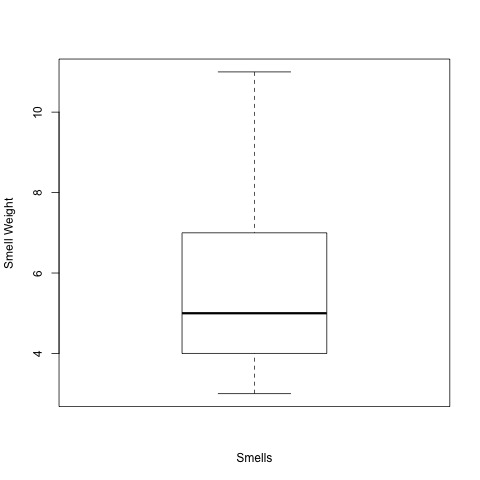
\epsfig{file = Bower_complex-chaining_rboxplot.jpg, width = 4cm}}%
	}
	\subfigure[Chart \newline \hspace*{0.5cm}Complex Code \newline \hspace*{0.5cm}Threshold: 34]{%
		{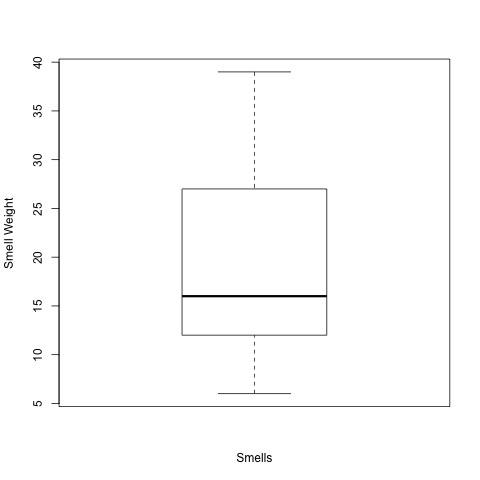
\epsfig{file = Chart_complexity_rboxplot.jpg, width = 4cm}}%
	}
	\subfigure[Express \newline \hspace*{0.5cm}Long Methods \newline \hspace*{0.5cm}Threshold: 44]{%
		{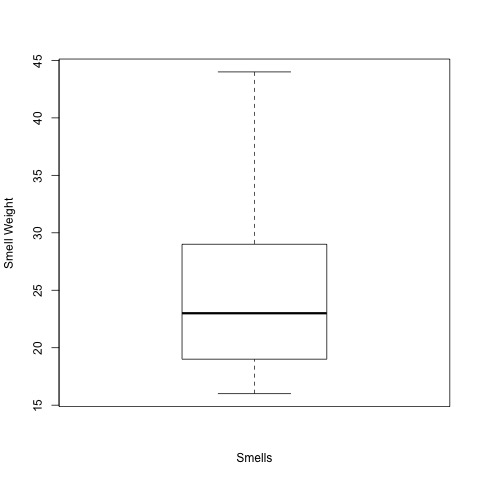
\epsfig{file = Express_max-statements_rboxplot.jpg, width = 4cm}}%
	}
	\subfigure[JQuery \newline \hspace*{0.5cm}Complex Switch Case \newline \hspace*{0.5cm}Threshold: 6]{%
		{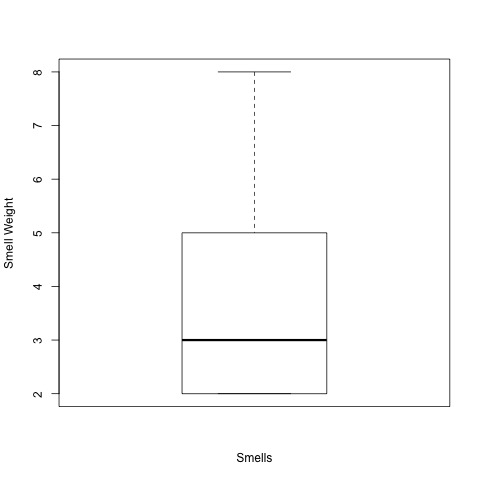
\epsfig{file = Jquery_complex-switch-case_rboxplot.jpg, width = 4cm}}%
	}
	\subfigure[Vue \newline \hspace*{0.5cm}Long Parameter List \newline \hspace*{0.5cm}Threshold: 9]{%
		{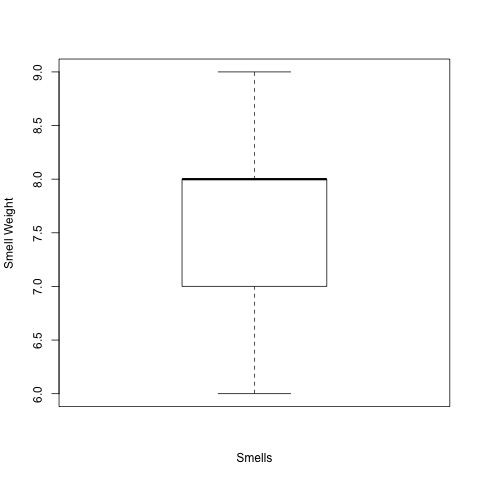
\epsfig{file = Vue_max-params_rboxplot.jpg, width = 4cm}}%
	}
	\subfigure[Ramda \newline \hspace*{0.5cm}Lengthy Lines \newline \hspace*{0.5cm}Threshold: 144]{%
		{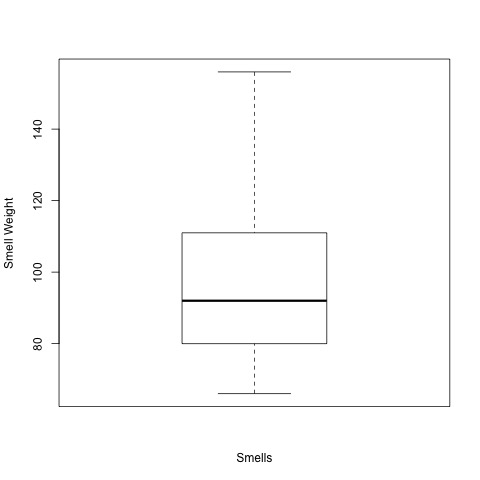
\epsfig{file = Ramda_max-len_rboxplot.jpg, width = 4cm}}%
	}
	\caption{Boxplots of some smells.\vspace{-10pt}}
	\label{boxplots}
\end{figure*}

\mytitle{Code Smell Detection} Among the 12 metric values reported by our framework, 4 are boolean. The boolean metrics concern \emph{This Assign}, \emph{Extra Bind}, \emph{Assignment in Conditional Statements}, and \emph{Variable Re-assign} smells. The 8 remaining metrics are integers. To identify code smells using the metric values provided by our framework, we follow the same approach as previous works~\cite{saboury2017empirical,marinescu2004detection, mazinanian2016migrating}, defining threshold values above which files should be considered as having the code smell. We define the thresholds relative to the systems using Box-plot analysis{\color{blue}, by being sure that all the chosen thresholds correspond to a smell population above the third quartile (75\%) in the boxplots. Figures~\ref{boxplots} show some relevant boxplots we found (meaning some with several values significantly taken by the smells), with the associated chosen threshold value in the title. All the boxplots appear in the Github repository of the project}. We chose to define threshold values relative to the projects because design rules and programming styles can vary from one project to another, and hence it is important to compare the characteristics of files in the context of the project. For each system, we obtain the threshold values as follows. We examined the distribution of the metrics and observed a big gap around the first 70\% of the data and the top 10\%. Hence, we decided to consider files with metric values in the top 10\% as containing the code smell. For files that contain multiple functions, we aggregated the metric values reported for each functions using the maximum to obtain a single value characterizing the file. {\color{blue}For our line grain analysis, since some smells (like long methods smells) appear on several consecutive lines, we record the lines range for these specific type smells, which is provided by the framework ESLint. For the other smells (like re-assign smells), we only report the line location). We manually examined a sample of JQuery project files marked as ``smelly" by our algorithm to verify that they are indeed smelly. Among almost 9000 smelly files reported by our algorithm, we randomly selected a sample of 100 files (to ensure a confidence interval of at least 90\%). We manually inspected the files and found that they all %, and notice that all these files are really smelly because they 
contain at least one smell with a weight above the chosen corresponding threshold.} %of the metric values reported for each function contained in the file to obtain a metric value characterizing the file.

%aformentioned In order to convert those numeric values into boolean which indicate the presence of a type of smell, we used a statistical approach to define the threshold . Since the culture, style guide and design rules could be different from a project to another, we defined the threshold specifically for each project in our case study.
%
%To define the threshold, we first removed the top 1\% of the data to remove extreme cases. By looking at the distribution of the numeric values of extracted metrics, for most of the metrics we saw there is a big gap around the first 70\% of the data and the top 10\%. So we considered the top 10\% of each metric as smelly codes. To analyze the sensitivity of the threshold to the result, we rerun our analysis with the threshold values of top 33\% and top 30\% as well and we observed no significant difference.
%Also as files could contain multiple functions and so multiple smelly parts, our framework could extract multiple values for each file for each numeric metric. To reduce this list of values to a single number, we get the maximum value of the list and associated that with the file.
%
%\section{Code Smells}\label{smells}
%Code smells are the results of bad design choices. They are referred to the structural characteristics in software code which could make the software harder to maintain or evolve \cite{fontana2012automatic}. Code smells usually the starting point of re-factoring \cite{fontana2012automatic, hamza2008code, fard2013jsnose}.

%\mytitle{Analysis}
%At the end, we feed the data to our R scripts to generate the result. We wrapped the R scripts into our framework to automate the whole process. In the following %section we will discuss about our analysis approach.

\subsection{Analysis}\label{survival}

{\color{blue}In this section, we detail the data analysis methods for each research question. Since Survival models are the cornerstone of our analysis, we first provide background information about them. % are used all along our data analysis, that is why we need to explain first what is the purpose of a survival analysis and how it works before precising the model analysis for each research question.
	
\textbf{Survival analysis} is used to model the time until the occurrence of a well-defined event~\cite{fox2010r}. One of the most popular models for survival analysis is the Cox Proportional Hazards (Cox) model. A Cox hazard model is able to model the instantaneous hazard of the occurrence of an event as a function of a number of independent variables~\cite{koru2008theory}~\cite{singer2003applied}. Particularly, Cox models aim to model how long subjects under observation can \textsl{survive} before the occurrence of an event of interest (\eg{} a fault occurrence or a smell occurence in our case) ~\cite{singer2003applied}~\cite{selim2010studying}.
	
Survival models were first introduced in demography and actuarial sciences~\cite{Westergaard}. Recently, researchers have started applying them to problems in the domain of Software Engineering. For example, Selim et al.~\cite{selim2010studying} used the Cox model to investigate characteristics of cloned code that are related to the occurrence of faults. Koru et al.~\cite{koru2007modeling} also used Cox models to analyze faults in software systems. %formulated the modeling by using Cox in order to find the effect of size on the defects.
In Cox models, the hazard of a fault occurrence at a time $t$ is modeled by the following function:
	
\begin{equation}\label{eq1}
\lambda_{i}(t) = \lambda_{0}(t)* e ^ {\beta*{F_{i}}(t)}
\end{equation}
	
If we take log from both sides, we obtain:
	
\begin{equation}\label{eq2}
log(\lambda_{i}(t)) = log(\lambda_{0}(t)) + {\beta_{1}*{f_{i1}}(t)} + ... + {\beta_{n}*{f_{in}}(t)}
\end{equation}
	
Where:
\begin{itemize}
	\item ${F_{i}}(t)$ is the time-dependent covariates of observation $i$ at the time $t$.
	\item $\beta$ is the coefficient of covariates in the function ${F_{i}}(t)$.	
	\item $\lambda_0$ is the baseline hazard.
	\item $n$ is the number of covariates.
\end{itemize}
	
When all the covariates have no effect on the hazard, the baseline hazard can be considered as the hazard of occurrence of the event (\eg{} a fault or a smell). The baseline hazard would be omitted when formulating the relative hazard between two files (in our case) at a specific time, as shown in the following Equation~\ref{eq3}.
	
\begin{equation}\label{eq3}
\lambda_{i}(t) \slash \lambda_{j}(t) = e ^ {\beta*{(f_{i}(t) - f_{j}(t))}}
\end{equation}
	
The proportional hazard model assumes that changing each covariate has the effect of multiplying the hazard rate by a constant.
	
%It is obvious that the relative hazard has nothing to do with the baseline hazard. This is called the proportional hazard assumption.
	
\textbf{Link function}. As Equation~(\ref{eq2}) shows, the log of the hazard is a linear function of the log of the baseline hazard and all the other covariates. In order to build a Cox proportional model, a linear relationship should be available between the log hazard and the covariates~\cite{therneau2000modeling}. Link functions are used to transform the covariates to a new scale if such relationship does not exist. Determining an appropriate link function for covariates is necessary because it allows changes in the original value of a covariate to influence the log hazard equally. This allows the proportionality assumption to be valid and applicable~\cite{therneau2000modeling}.
	
\textbf{Stratification}. In addition to applying a link function, a stratification is sometimes necessary to preserve the proportionality in Cox hazard models \cite{koru2008theory}. For example, if there is a covariate that needs to be controlled because it is of no interest or secondary, stratification can be used to split the data set so that the influence of more important covariates can be monitored better \cite{koru2008theory}.
	
\textbf{Model validation}. Since Cox proportional hazard models assume that all covariates are consistent over time and the effect of a covariate does not fluctuate with time, hence, to validate our model, we apply a non-proportionality test to ensure that the assumption is satisfied~\cite{selim2010studying}\cite{therneau2000modeling}.
	
In this paper, we perform each of our analysis {\color{blue} on each file of each commit of the studied projects, and refine the correlations between faults and smells experienced by a file with our line grain analysis.} Then, for each file, we use Cox proportional hazard models to calculate the risk of a fault or a smell occurrence over time, considering a number of independent covariates. We chose the Cox proportional hazard model for the following reasons:\\
(1) In general, not all files in a commit experience a fault. Cox hazard models allow files to remain in the model for the entire observation period, even if they don't experience the event (\ie{} fault occurrence). (2) In Cox hazard models, subjects can be grouped according to a covariate (\eg{} smelly or non-smelly). (3) The characteristics of the subjects might change during the observation period (\eg{} size of code), and (4) Cox hazard models are adapted for events that are recurrent~\cite{therneau2000modeling}, which is important because software modules evolve over time and a file can have multiple faults during its life cycle.
	
\subsubsection*{(RQ1) Is the risk of fault higher in files with code smells in comparison with those without code smell?}\label{AnalysisRQ1}

To assess the impact of code smells on the fault-proneness of JavaScript files, we perform survival analysis, comparing the time until a fault occurrence, in files containing code smells {\color{blue} with match between faulty and smelly lines}, and files without code smells. %{\color{blue}(including files with code smells but no match between faulty and smelly lines)}.
For each file and for each revision $r$ (\ie{} corresponding to a commit), we also compute the following metrics:
\begin{itemize}
	\item \textbf{Time:} the number of hours between the previous revision of the file and the revision $r$.
	We set the time of the first revision to zero.
	\item \textbf{Smelly:} this is our covariate of interest. It takes the value $1$ if the revision $r$ of the file contains a code smell and $0$ if it doesn't contain any of the 12 studied code smells.
	\item \textbf{Event:} For the line grain analysis (respectively the line grain analysis including dependencies), this metric takes the value $1$ if the revision $r$ is a fault-fixing change and if there is at least one match between the faulty lines (respectively the extended faulty lines described in Section~\ref{extraction}) and the code smell lines, and $0$ otherwise. Indeed, if there is no matching, we consider that the fault-fixing change doesn't relate to code smells. We use the improved SZZ algorithm to insure that the file contained a code smell when the fault was introduced.
\end{itemize}

Using the smelly metric, we divide our dataset in two groups: one group containing files with code smells (\ie{} smelly = 1) and another group containing files without any of the 12 studied code smells (\ie{} smelly = 0). For each group we create an individual Cox hazard model. In each group, the covariate of interest (\ie{} smelly) is a constant function (with value either 1 or 0), hence, there is no need for a link function to establish a linear relationship between this covariate and our event of interest, \ie{} the occurrence of a fault. We use the \textsl{survfit} and \textsl{coxph} functions from R~\cite{rPackage} to analyze our Cox hazard models.

In addition to building Cox hazard models, we test the following null hypothesis: \emph{$H^{1}_{0}$: There is no difference between the probability of a fault occurrence in a file containing code smells and a file without code smells}. We use the \textsl{log-rank} test (which compares the survival distributions of two samples), to accept or refute this null hypothesis.

\subsection*{(RQ2) Are JavaScript files with code smells equally fault-prone?}\label{AnalysisRQ2}

Similar to \textbf{RQ1}, for each file and for each revision $r$ (\ie{} corresponding to a commit), we compute the \textbf{Time} and \textbf{Event} metrics defined in \textbf{RQ1}. For each type of code smell $i$ we define the metric \textbf{Smelly$_{i}$:} which takes the value $1$ if the revision $r$ of the file contains the code smell $i$ and $0$ if it doesn't contain any of the 12 studied code smells. Also, similarly to \textbf{RQ1}, for the line grain analysis (respectively the line grain analysis including dependencies), we define the metric \textbf{Event$_{i}$:} which takes the value $1$ if the revision $r$ is a fault-fixing change and if the code smell $i$ is in the intersection between  the faulty lines (respectively the extended faulty lines described in Section~\ref{extraction}) and the smelly lines, and $0$ otherwise. When computing the \textbf{Event} and the \textbf{Event$_{i}$} metrics, we used the improved SZZ algorithm to ensure that the file contained the code smell $i$ when the fault was introduced. % (zero or one) whether the change has any code smell or not.
Because size, code churn, and the number of past occurrence of faults are known to be related to fault-proneness, we add the following metrics to our models, to control for the effect of these covariates : (i) LOC: the number of lines of code in the file at revision $r$; (ii) Code Churn: the sum of added, removed and modified lines in the file prior to revision $r$; (iii) No. of Previous-Bugs: the number of fault-fixing changes experienced by the file prior to revision $r$.

%
%To specify which covariates play significant roles in reaching a defect, we fetched all the data considering all 12 types of code smells. We also consider metrics such as LOC, code churn and the number of previous defects that the file had before. To that end, we create another data set involving all of these covariates as the columns. Similar to our previous approach, we collect the observations on our data set based on the following fields:
%
%1) Time: The number of hours between the previous revision to and either 1) this revision or 2) the end of the study, whichever occurs first. The Start time of the first revision is set to zero.
%
%2) No. of Previous-Bugs: The covariate of interest (zero or more) of how many times this file at this revision had a bug fix before.
%
%3) to (14) 12 columns including each code smell type (e.g., \textsl{max-len}, \textsl{this assign}, etc.): The covariates of interest (zero or one) of whether the file has this specific type of code smell or not. If so, the corresponding column would be 1, otherwise 0.
%
%15) LOC: The covariate of interest which holds the number of lines of code. LOC often changes during each revision.
%16) Code Churn: The covariate of interest which holds the summation of lines added and removed at this revision.
%17) Event: An indicator (zero or one) of whether this is a defect-fixing revision.
We perform a stratification considering the covariates mentioned above, in order to monitor their effect on our event of interest, \ie{} a fault occurrence. Next, we create a Cox hazard model for each of our fifteen studied systems.
In order to build an appropriate link function for the new covariates considered in this research question (\ie{} LOC, Code churn, and No. of Previous-Bugs), we follow the same methodology as ~\cite{koru2008theory}~\cite{selim2010studying} and plot the log relative risk vs. each type of code smell, the No. of Previous-Bugs, LOC and Code Churn in each of our fifteen datasets (corresponding to the fifteen subject systems). We generated summaries of all our Cox models and removed insignificant covariates, \ie{} those with $p$-values greater than $0.05$. Finally, for each system, we performed a non-proportional test to verify if the proportional hazards assumption holds.

\subsection*{(RQ3) How long do code smells survive in JavaScript projects?}\label{AnalysisRQ3}

To assess the impact of smells survival over project lifetime, we perform survival analysis, comparing the time between the creation of a type of code smell and either their removal, or the last revision of the studied projects. %comparing the time until a type smell occurrence in files containing code smells, for each of the 12 studied type smell.}\\
For each studied system and for each smell type, we compute the following metrics:
\begin{itemize}
	\item The number of created smells.
	\item The number of killed smells (over the system lifetime).
	\item The number of survived smells, which means the number of smell that are still in the system.
	\item The number of smells created at the file birthdate.
	\item The median days of survival of the smells.
	\item The average days of survival of the smells.
\end{itemize}
For each smell created (which means that it was never encountered before), we also compute the \textbf{Time} and \textbf{Event} metrics defined below:
\begin{itemize}
	\item \textbf{Time:} the time in days since the smell creation.
	\item \textbf{Event:} this metric takes the value $1$ if the studied smell is present at this time (which means that it has not been removed), and $0$ otherwise.
\end{itemize}
In this way, if a particular smell $s$ is removed $x$ days after its introduction, we will have the corresponding event metric equal to $1$ from $0$ to $x-1$, and equal to $0$ at the time $x$ and after. When we report these informations for a studied system, the maximum time that we take in account, for a particular smell type, corresponds to the maximum lifetime of the smells of this type. Thereby, for each smell type of the system and for each time, we will know the proportion of smells alive relatively to the number of smells created. This will particularly help us in the Cox survival model design.

Similar to \textbf{RQ1}, for each of the twelve studied smells, and for each of the fifteen studied systems, we create an individual Cox survival model using the \textbf{Time} and \textbf{Event} metrics defined above. We use the \textsl{survfit} and \textsl{coxph} functions from R~\cite{rPackage} to analyze our Cox survival models.}


\section{Case Study Results}\label{sec:case-study}
In this section, we report and discuss the results for each research question.
%{\color{blue}For each research question, we collect information about smell, and fault hazard codes of JavaScript files of the studied systems, and more specifically those which end with the \textsl{.js} extension. Also, we don't take in account the JavaScript files with \textsl{.min.js} extension, because they are a minified version of \textsl{.js} files that we already keep in our study. In this way, we avoid redundancy in our analyzes.}

\subsection*{(RQ1) Is the risk of fault higher in files with code smells in comparison with those without code smell?}

%\textbf{Motivation}. Code smells are poor solutions in software design and implementation problems. Previous studies such as Jaafar et al.~\cite{jaafar2013mining} has shown that the fault-proneness of modules are significantly different between implementations with code smells and implementations without them. As stated by ~\cite{jaafar2013mining}: ``classes having dependencies with anti-patterns are more fault-prone than others". However, their study has been done on Java software systems. To the best of our knowledge, less is known on the code smells of JavaScript. Hence, in this research question we aim to explore how code smells affect the reliability of a software developed in JavaScript.

%This knowledge helps software practitioners plan to detect the code smells as much early as possible in the very beginning phase of software development before the code base gets %bigger.%

\begin{table*}[t]
	\centering
	\scriptsize
	\caption{Fault hazard ratios for each project with the line grain approach. $exp(coef)$ values means higher hazard rates.}
	\label{hazardlinegrain}
	\begin{tabular}{l|l|l|l}
		\hline
		module & $exp(coef)$ & $p$-value (Cox hazard model) & $p$-value (Proportional hazards assumption)     \\ \hline
		express  & 1.603 & 4.415e-08 & 0.046 \\ \hline
		request  & 2.328 & 3.737e-4 & 0.977 \\ \hline
		less  & 1.801 & 7.896e-7 & 0.085 \\ \hline
		bower	 & 1.512 & 6.833e-5 & 0.826 \\ \hline
		grunt    & 0.994 & 0.961 & 0.068 \\ \hline
		jquery	 & 3.091 & 0 & 1.294e-11 \\ \hline
		vue   & 0.110 & 0 & 0.001 \\ \hline
		ramda 	 & 0.780 & 0.020 & 0.390 \\ \hline
		leaflet	 & 0.707 & 6.076e-9 & 0.752 \\ \hline
		hexo	 & 1.439 & 2.891e-5 & 0.700 \\ \hline
		chart	 & 1.043 & 0.771 & 0 \\ \hline
		webpack	 & 1.134 & 0.006 & 0 \\ \hline
		webtorrent & 1.444 & 0.180 & 0.814 \\ \hline
		moment	 & 0.996 & 0.954 & 1.878e-7 \\ \hline
		riot	 & 0.973 & 0.717 & 0.167 \\ \hline
	\end{tabular}

\end{table*}

\begin{figure*}[t]
	\centering%
	\subfigure[express.js]{%
		{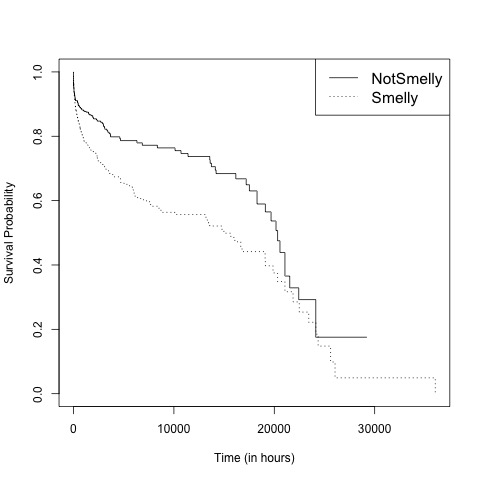
\epsfig{file = Express_bugs_smells_line-grain_large_rplot.jpg, width = 3.5cm}}%
	}
	\subfigure[request.js]{%
		{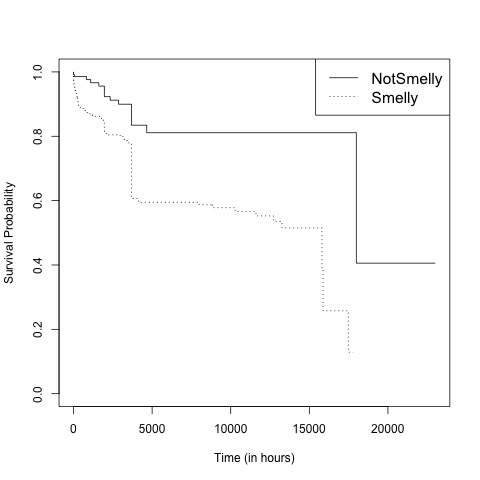
\epsfig{file = Request_bugs_smells_line-grain_large_rplot.jpg, width = 3.5cm}}%
	}
	\subfigure[less.js]{%
		{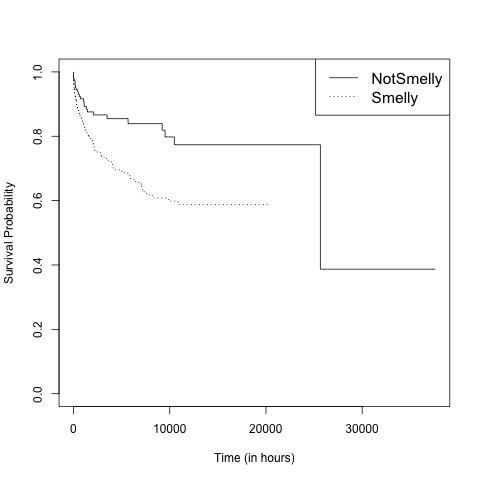
\epsfig{file = Less_bugs_smells_line-grain_large_rplot.jpg, width = 3.5cm}}%
	}
	\subfigure[grunt.js]{%
		{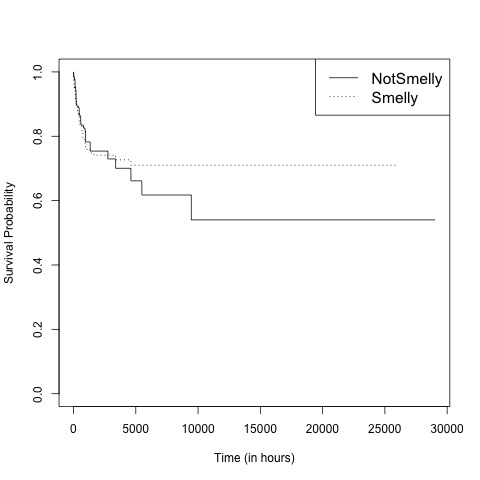
\epsfig{file = Grunt_bugs_smells_line-grain_large_rplot.jpg, width = 3.5cm}}%
	}
	\subfigure[bower.js]{%
		{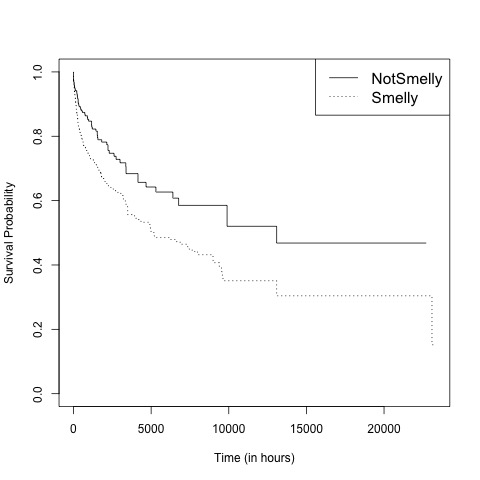
\epsfig{file = Bower_bugs_smells_line-grain_large_rplot.jpg, width = 3.5cm}}%
	}
	\subfigure[jquery.js]{%
		{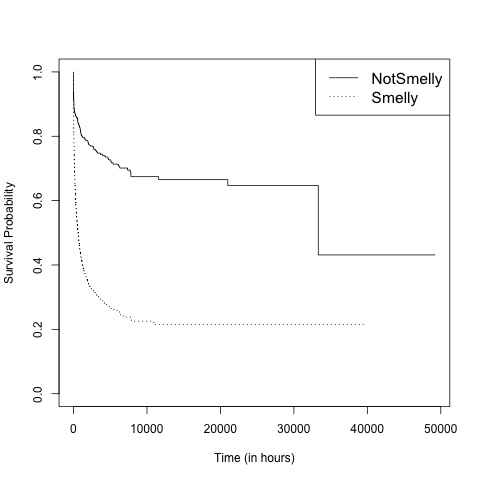
\epsfig{file = Jquery_bugs_smells_line-grain_large_rplot.jpg, width = 3.5cm}}%
	}
	\subfigure[hexo.js]{%
		{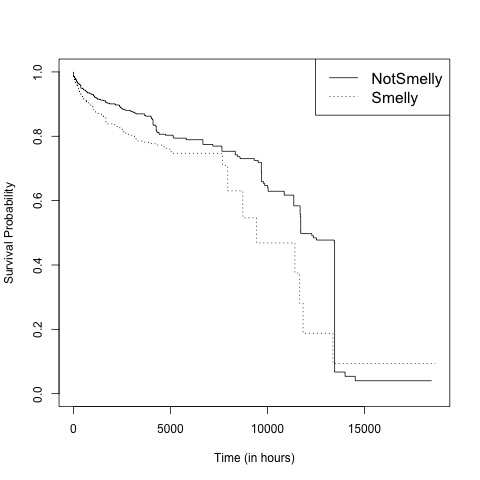
\epsfig{file = Hexo_bugs_smells_line-grain_large_rplot.jpg, width = 3.5cm}}%
	}
	\subfigure[leaflet.js]{%
		{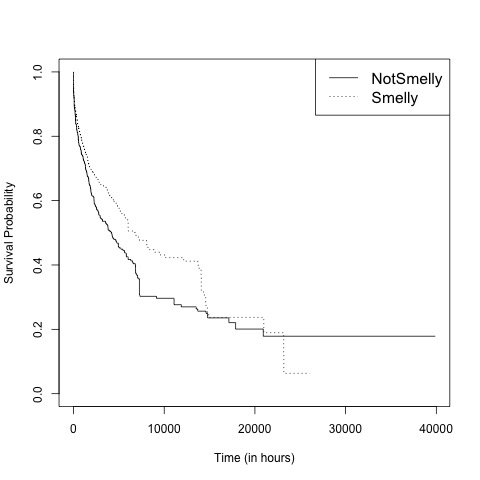
\epsfig{file = Leaflet_bugs_smells_line-grain_large_rplot.jpg, width = 3.5cm}}%
	}
	\subfigure[ramda.js]{%
		{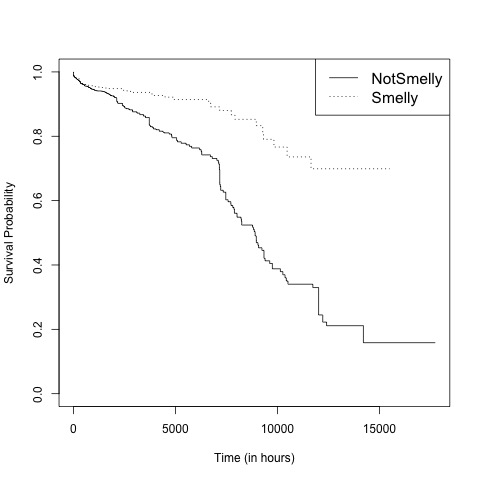
\epsfig{file = Ramda_bugs_smells_line-grain_large_rplot.jpg, width = 3.5cm}}%
	}
	\subfigure[chart.js]{%
		{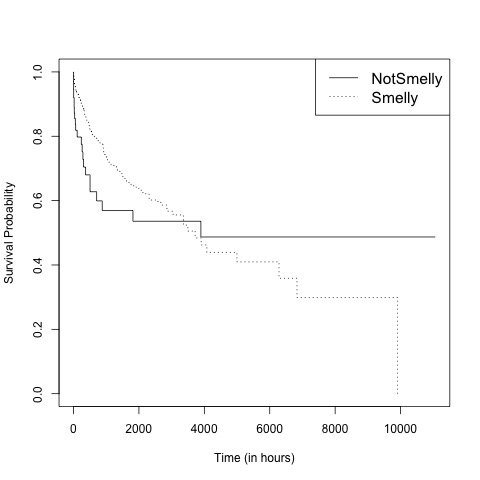
\epsfig{file = Chart_bugs_smells_line-grain_large_rplot.jpg, width = 3.5cm}}%
	}
	\subfigure[riot.js]{%
		{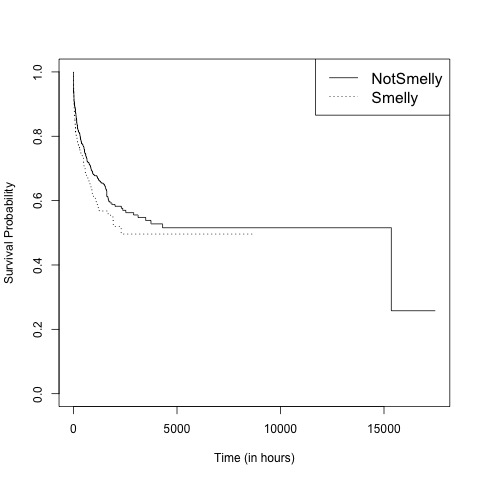
\epsfig{file = Riot_bugs_smells_line-grain_large_rplot.jpg, width = 3.5cm}}%
	}
	\subfigure[vue.js]{%
		{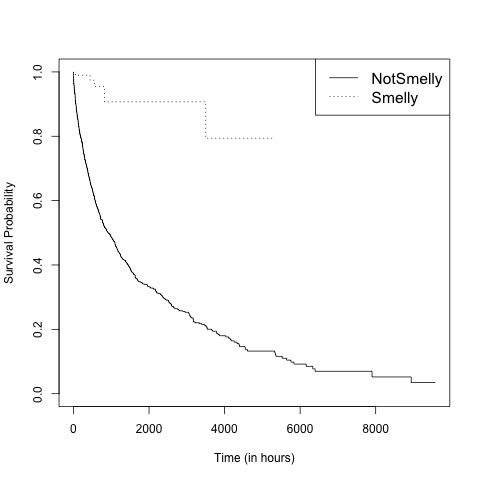
\epsfig{file = Vue_bugs_smells_line-grain_large_rplot.jpg, width = 3.5cm}}%
	}
	\subfigure[moment.js]{%
		{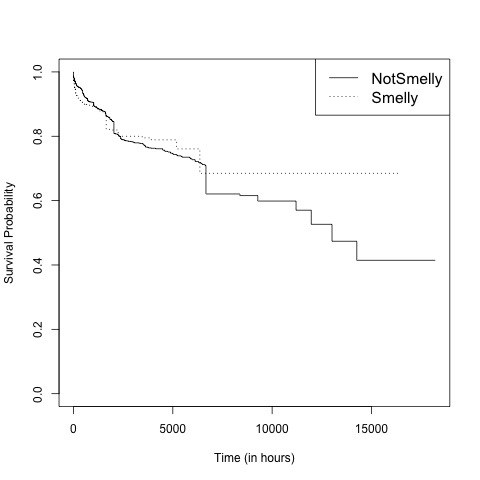
\epsfig{file = Moment_bugs_smells_line-grain_large_rplot.jpg, width = 3.5cm}}%
	}
	\subfigure[webpack.js]{%
		{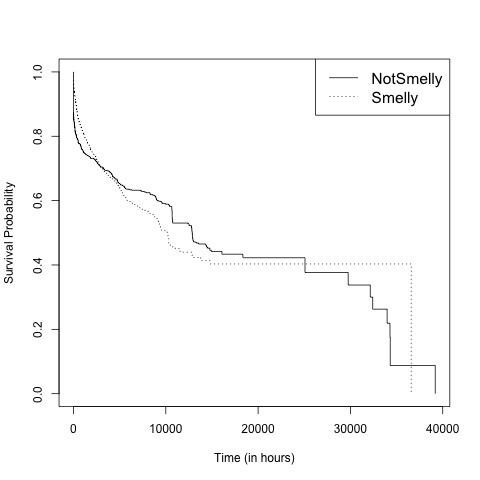
\epsfig{file = Webpack_bugs_smells_line-grain_large_rplot.jpg, width = 3.5cm}}%
	}
	\subfigure[webtorrent.js]{%
		{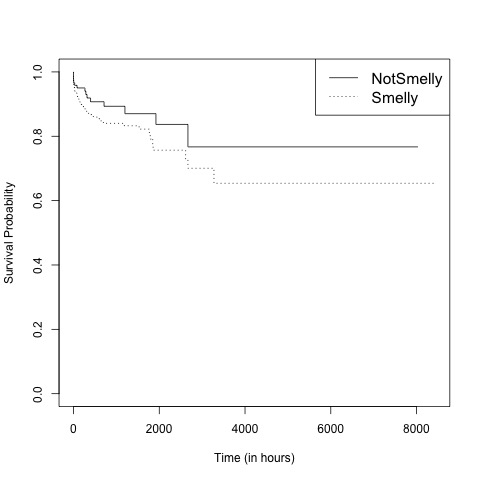
\epsfig{file = Webtorrent_bugs_smells_line-grain_large_rplot.jpg, width = 3.5cm}}%
	}
	\caption{Survival probability trends of smelly codes vs. non-smelly codes in our fifteen JavaScript projects with the line grain including dependencies approach.\vspace{-10pt}}
	\label{rq1-2}
\end{figure*}

\textbf{Approach}. We use our framework described in Section~\ref{extraction} (Figure~\ref{process}) to collect information about the occurrence of the 12 studied code smells in our fifteen subject systems. %fetch all the data considering all 12 types of code smells.
Then, we apply the data analysis model described in Section~\ref{AnalysisRQ1} (RQ1) to our collected data.

\textbf{Findings}. Table~\ref{hazardlinegrain} (line grain results) and Figure~\ref{rq1-2} (line grain including dependencies results) show that files containing code smells experience faults faster than files without code smells, which confirms the finding of Saboury et al.~\cite{saboury2017empirical} obtained at the file level, {\color{blue}without matching faulty and smelly code lines}. The $Y$-axis in Figure~\ref{rq1-2} represents the probability of a file experiencing a fault occurrence. Hence, a low value on the $Y$-axis means a low \emph{survival} rate (\ie{} a high hazard or high risk of fault occurrence).
For all fifteen projects, we calculated relative hazard rates (using Equation~(\ref{eq3}) from Section~\ref{survival}) between files containing code smells and files without code smells. Results show that, on average, files without code smells have hazard rates 33\% lower than files with code smells in our line grain analysis, and 45\% lower in our line grain analysis considering dependencies. It is normal to see this proportion decreasing in line grain analysis (in comparison with the file grain analysis of Saboury et al.~\cite{saboury2017empirical}), because we add an additional matching condition to set the \emph{event} to $1$. Between the line grain analysis and the line grain including dependencies analysis, the proportion increased slightly because considering dependencies increases the number of faulty lines that are related to code smells. We performed a \textsl{log-rank} test comparing the survival distributions of files containing code smells and files without any of the studied code smells and obtained $p$-values lower than $0.05$ for most of the fifteen studied systems. Hence, we reject $H^{1}_{0}$.
Since our detection of code smells depends on our selected threshold value (\ie{} the top 10\% value chosen in Section~\ref{extraction}), we conducted a sensitivity analysis to assess the potential impact of this threshold selection on our result. More specifically, we rerun all our analysis with threshold values at top 20\% and top 30\%. We observed no significant differences in the results. Hence, we conclude that:

\hypobox{JavaScript files without code smells have hazard rates 33\% lower than JavaScript files with code smells when considering fault occurrences on code smell lines (\ie{} the line grain granularity), and this difference is statistically significant. If we consider the extended candidate fault lines described in Section~\ref{extraction} the hazard rate increases to 45\%.} %Plus, this difference still remains significant and increases in the line grain including dependencies approach, because hazard rates reach 45\%.}}

{\color{blue}JavaScript developers should be careful to avoid introducing code smells because they increase the probability of introducing faults. Also, refactoring should be considered to remove code smells since it could help reduced the fault-proneness of the systems.}

\subsection*{(RQ2) Are JavaScript files with code smells equally fault-prone?}

%\begin{table*}[t]
%\centering%
%\caption{Covariates coeffiecients on the defects. Higher exp(coef) means higher hazard rate.}
%\begin{tabular}{c|c|c|c|c|c|c}
%\hline
%module & covariate & exp(coef) & se(coef) & z & p & Non-proportionality test (p-value) \\ \hline
%\multirow{3}{*}{express} & No.Previous-Bugs & 1.01842956 & 0.00300334 & 6.08 & 0.0000000012 & 0.887 \\ \cline{2-7}
% & cond.assign & 1.55093782 & 0.14811000 & 2.96 & 0.0030 & 0.561 \\ \cline{2-7}
% & LOC & 1.00111187 & 0.00019567 & 5.68 & 0.0000000135 & 0.382 \\ \hline
%\multirow{2}{*}{grunt} & cond.assign & 2.36768081 & 0.24248431 & 3.55 & 0.00038 & 0.2237 \\ \cline{2-7}
% & nested.callbacks & 3.13565940 & 0.41026000 & 2.79 & 0.00534 & 0.8147 \\ \hline
%\multirow{3}{*}{bower} & No.Previous-Bugs & 1.025646 & 0.007863 & 3.22 & 0.0013 & 0.415 \\ \cline{2-7}
% & max.depth & 9.222632 & 0.452966 & 4.90 & 0.00000094 & 0.960 \\ \cline{2-7}
% & LOC & 1.000643 & 0.000295 & 2.18 & 0.0295 & 0.414 \\ \hline
%\multirow{3}{*}{less} & No.Previous-Bugs & 1.036634202 & 0.003126697 & 11.51 & 0.000002 & 0.739 \\ \cline{2-7}
% & complex.switch.case & 0.484588521 & 0.332039480 & -2.18 & 0.02912 & 0.4177 \\ \cline{2-7}
% & cond.assign & 1.664212015 & 0.131560216 & 3.87 & 0.00011 & 0.9154 \\ \hline
%\multirow{3}{*}{request} & No.Previous-Bugs & 1.0675617 & 0.0218429 & 2.99 & 0.0028 & 0.4074 \\ \cline{2-7}
% & max.depth & 0.1723391 & 0.4346634 & -4.05 & 0.000052 & 0.6207 \\ \cline{2-7}
% & LOC & 1.0009179 & 0.0003798 & 2.42 & 0.0157 & 0.8668 \\ \hline
%\end{tabular}
%\end{table*}

% Please add the following required packages to your document preamble:
% \usepackage{multirow}
%\begin{table*}[t]
%\centering%
%\caption{Covariates coeffiecients on the defects. Higher exp(coef) means higher hazard rate.}
%\begin{tabular}{c|c|c|c|c}
%\hline
%module & covariate & exp(coef) & p & Non-proportionality test (p-value) \\ \hline
%\multirow{3}{*}{express} & No.Previous-Bugs & 1.01842956 & 0.0000000012 & 0.887 \\ \cline{2-5}
% & cond.assign & 1.55093782 & 0.0030 & 0.561 \\ \cline{2-5}
% & LOC & 1.00111187 & 0.0000000135 & 0.382 \\ \hline
%\multirow{2}{*}{grunt} & cond.assign & 2.36768081 & 0.00038 & 0.2237 \\ \cline{2-5}
% & nested.callbacks & 3.13565940 & 0.00534 & 0.8147 \\ \hline
%\multirow{3}{*}{bower} & No.Previous-Bugs & 1.025646 & 0.0013 & 0.415 \\ \cline{2-5}
% & max.depth & 9.222632 & 0.00000094 & 0.960 \\ \cline{2-5}
% & LOC & 1.000643 & 0.0295 & 0.414 \\ \hline
%\multirow{3}{*}{less} & No.Previous-Bugs & 1.036634202 & 0.000002 & 0.739 \\ \cline{2-5}
% & complex.switch.case & 0.484588521 & 0.02912 & 0.4177 \\ \cline{2-5}
% & cond.assign & 1.664212015 & 0.00011 & 0.9154 \\ \hline
%\multirow{3}{*}{request} & No.Previous-Bugs & 1.0675617 & 0.0028 & 0.4074 \\ \cline{2-5}
% & max.depth & 0.1723391 & 0.000052 & 0.6207 \\ \cline{2-5}
% & LOC & 1.0009179 & 0.0157 & 0.8668 \\ \hline
%\end{tabular}
%\end{table*}

% Please add the following required packages to your document preamble:
% \usepackage{multirow}
\begin{table}[t]
	\centering
	\scriptsize
	\caption{Hazard ratios for each type of code smells (for the line grain analysis). Higher $exp(coef)$ values means higher hazard rates.}
	\begin{tabular}{c|c|c|p{1.1cm}|p{1.3cm}}
		\hline
		module & covariate & $exp(coef)$ & $p$-value (Cox hazard model) & $p$-value (Proportional hazards assumption) \\ \hline
		\multirow{2}{*}{express}
		& No.Previous-Bugs & 1.030 & 0 & 0.244 \\ \cline{2-5}
		& Code Churn & 1 & 0.677 & 0.688 \\ \cline{2-5}
		& LOC & 1.002 & 0 & 0.02 \\ \cline{2-5}
		& Variable Re-assign & 1.45 & 6.681e-6 & 0.265  \\ \hline
		\multirow{4}{*}{grunt}
		& No.Previous-Bugs & 1.017 & 9.883e-5 & 0.445 \\ \cline{2-5}
		& Code Churn & 0.999 & 0.375 & 0.77 \\ \cline{2-5}
		& LOC & 1 & 0.649 & 0.586 \\ \cline{2-5}
		& Assign. in Cond. State. & 0.509 & 0.0346 & 0.349 \\ \cline{2-5}
		& Chained Methods & 0.42 & 4.479e-4 & 0.44 \\ \cline{2-5}
		& Lengthy Lines & 0.408 & 8.779e-6 & 0.597 \\ \hline
		\multirow{4}{*}{bower}
		& No.Previous-Bugs & 1.053 & 0 & 0.559 \\ \cline{2-5}
		& Code Churn & 1 & 0.639 & 0.028 \\ \cline{2-5}
		& LOC & 1.001 & 1.01e-14 & 0.477 \\ \cline{2-5}
		& Variable Re-assign & 1.556 & 1.392e-5 & 0.679 \\ \cline{2-5}
		& This Assign & 0.583 & 3.399e-5 & 0.034 \\ \hline
		\multirow{3}{*}{less}
		& No.Previous-Bugs & 1.022 & 0 & 0.373 \\ \cline{2-5}
		& Code Churn & 0.999 & 8.959e-4 & 0.456 \\ \cline{2-5}
		& LOC & 1 & 1.059e-5 & 0.197 \\ \cline{2-5}
		& Variable Re-assign & 1.638 & 1.658e-5 & 0.039 \\ \cline{2-5}
		& Assign. in Cond. State. & 1.263 & 0.056 & 0.953 \\ \hline
		\multirow{3}{*}{request}
		& No.Previous-Bugs & 1.06 & 0 & 0.496 \\ \cline{2-5}
		& Code Churn & 1 & 0.928 & 0.748 \\ \cline{2-5}
		& LOC & 1.001 & 0 & 0.772 \\ \cline{2-5}
		& This Assign & 1.422 & 0.053 & 0.858 \\ \cline{2-5}
		& Variable Re-assign & 1.92 & 0.002 & 0.752 \\ \hline
		\multirow{4}{*}{jquery}
		& Code Churn & 1 & 2.237e-4 & 2.021e-14 \\ \cline{2-5}
		& LOC & 1 & 0 & 0.125 \\ \cline{2-5}
		& Lengthy Lines & 1.524 & 0 & 0.422 \\ \cline{2-5}
		& Assign. in Cond. State. & 1.414 & 0.001 & 0.016 \\ \cline{2-5}
		& Complex Code & 1.283 & 1.39e-5 & 0.911 \\ \hline
		\multirow{2}{*}{hexo}
		& No.Previous-Bugs & 1.197 & 0 & 0.05 \\ \cline{2-5}
		& Code Churn & 1.001 & 0.005 & 0.271 \\ \cline{2-5}
		& LOC & 1.001 & 0 & 0.082 \\ \cline{2-5}
		& Complex Code & 1.59 & 0.0756 & 0.247 \\ \cline{2-5}
		& Long Methods & 1.357 & 0.214 & 0.554 \\ \hline
		\multirow{5}{*}{leaflet}
		& No.Previous-Bugs & 1.015 & 0 & 0.017 \\ \cline{2-5}
		& Code Churn & 1 & 0.708 & 1.327e-4 \\ \cline{2-5}
		& LOC & 1.0001 & 1.108e-6 & 0.124 \\ \cline{2-5}
		& Variable Re-assign & 0.701 & 2.436e-9 & 0.567 \\ \cline{2-5}
		& Complex Code & 0.472 & 6.459e-4 & 0.048 \\ \cline{2-5}
		& Chained Methods & 0.462 & 8.513e-6 & 0.77 \\ \hline
		\multirow{4}{*}{ramda}
		& Code Churn & 1 & 0.619 & 0.436 \\ \cline{2-5}
		& LOC & 1 & 0.002 & 0.328 \\ \cline{2-5}
		& Nested Callbacks & 0.364 & 5.916e-6 & 0.004 \\ \cline{2-5}
		& Complex Code & 0.603 & 0.475 & 0.446 \\ \cline{2-5}
		& Chained Methods & 0.261 & 0.021 & 0.582 \\ \hline
		\multirow{4}{*}{chart}
		& No.Previous-Bugs & 1.056 & 0 & 0.993 \\ \cline{2-5}
		& Code Churn & 1 & 0.563 & 0.102 \\ \cline{2-5}
		& LOC & 1 & 0.466 & 0.454 \\ \cline{2-5}
		& Nested Callbacks & 0.287 & 0 & 5.257e-8 \\ \cline{2-5}
		& This Assign & 0.404 & 0 & 3.453e-6 \\ \cline{2-5}
		& Long Parameter List & 0.248 & 4.915e-9 & 0.057 \\ \hline
		\multirow{2}{*}{riot}
		& Code Churn & 0.994 & 4.415e-7 & 0.267 \\ \cline{2-5}
		& LOC & 1 & 8.598e-5 & 0.555 \\ \cline{2-5}
		& Variable Re-assign & 1.02 & 0.794 & 0.103 \\ \cline{2-5}
		& This Assign & 0.135 & 4.648e-11 & 0.131 \\ \cline{2-5}
		& Nested Callbacks & 0.244 & 0.047 & 0.036 \\ \hline
		\multirow{2}{*}{vue}
		& Code Churn & 0.998 & 1.464e-7 & 0.146 \\ \cline{2-5}
		& LOC & 1 & 1.11e-16 & 0.03 \\ \cline{2-5}
		& Variable Re-assign & 0.083 & 0 & 0.035 \\ \cline{2-5}
		& This Assign & 0.018 & 1.399e-8 & 0.145 \\ \hline
		\multirow{2}{*}{moment}
		& No.Previous-Bugs & 1.015 & 0 & 0.474 \\ \cline{2-5}
		& Code Churn & 1 & 0.17 & 0.442 \\ \cline{2-5}
		& LOC & 1 & 0.383 & 0.969 \\ \cline{2-5}
		& Complex Switch Case & 2.849 & 9.324e-7 & 0.925 \\ \cline{2-5}
		& Long Methods & 1.061 & 0.776 & 0.698 \\ \hline
		\multirow{1}{*}{webpack}
		& Code Churn & 1 & 0.622 & 7.173e-6 \\ \cline{2-5}
		& LOC & 1 & 0.44 & 0 \\ \cline{2-5}
		& Variable Re-assign & 1.131 & 0.008 & 0 \\ \cline{2-5}
		& Extra Bind & 0.554 & 0.238 & 0.628 \\ \hline
		\multirow{3}{*}{webtorrent}
		& No.Previous-Bugs & 1.043 & 1.576e-5 & 0.27 \\ \cline{2-5}
		& Code Churn & 1 & 0.997 & 0.441 \\ \cline{2-5}
		& LOC & 1.001 & 7.963e-4 & 0.257 \\ \cline{2-5}
		& Variable Re-assign & 1.488 & 0.114 & 0.637 \\ \cline{2-5}
		& Nested Callbacks & 0.258 & 0.02 & 0.761 \\ \hline
	\end{tabular}
	\label{smelltypes}
	\vspace{-15pt}
\end{table}

\begin{table}[t]
	\centering
	\scriptsize
	\caption{Hazard ratios for each type of code smells (for the line grain analysis that consider dependencies). Higher $exp(coef)$ values means higher hazard rates.}
	\begin{tabular}{c|c|c|p{1.1cm}|p{1.3cm}}
		\hline
		module & covariate & $exp(coef)$ & $p$-value (Cox hazard model) & $p$-value (Proportional hazards assumption) \\ \hline
		\multirow{4}{*}{express}
		& No.Previous-Bugs & 1.03 & 0 & 0.237 \\ \cline{2-5}
		& Code Churn & 1 & 0.542 & 0.695 \\ \cline{2-5}
		& LOC & 1.002 & 0 & 0.01 \\ \cline{2-5}
		& Complex Code & 3.504 & 0 & 0.184 \\ \cline{2-5}
		& Long Methods & 2.972 & 4.857e-12 & 0.25 \\ \cline{2-5}
		& Variable Re-assign & 1.572 & 2.581e-8 & 0.371 \\ \hline
		\multirow{2}{*}{grunt}
		& No.Previous-Bugs & 1.018 & 8.412e-6 & 0.495 \\ \cline{2-5}
		& Code Churn & 0.999 & 0.293 & 0.691 \\ \cline{2-5}
		& LOC & 1 & 0.787 & 0.542 \\ \cline{2-5}
		& Variable Re-assign & 1.123 & 0.284 & 0.079 \\ \cline{2-5}
		& Complex Code & 1.275 & 0.191 & 0.949 \\ \hline
		\multirow{4}{*}{bower}
		& No.Previous-Bugs & 1.05 & 0 & 0.597 \\ \cline{2-5}
		& Code Churn & 1 & 0.972 & 0.017 \\ \cline{2-5}
		& LOC & 1.001 & 0 & 0.58 \\ \cline{2-5}
		& Long Methods & 2.664 & 7.421e-10 & 0.478 \\ \cline{2-5}
		& Complex Code & 1.768 & 0.001 & 0.966 \\ \cline{2-5}
		& Variable Re-assign & 1.72 & 7.232e-8 & 0.954 \\ \hline
		\multirow{2}{*}{less}
		& No.Previous-Bugs & 1.022 & 0 & 0.312 \\ \cline{2-5}
		& Code Churn & 0.999 & 6.801e-4 & 0.457 \\ \cline{2-5}
		& LOC & 1 & 2.068e-5 & 0.172 \\ \cline{2-5}
		& Variable Re-assign & 1.74 & 1.102e-6 & 0.049 \\ \cline{2-5}
		& Assign. in Cond. State. & 1.37 & 0.008 & 0.973 \\ \hline
		\multirow{3}{*}{request}
		& No.Previous-Bugs & 1.055 & 0 & 0.544 \\ \cline{2-5}
		& Code Churn & 1 & 0.785 & 0.595 \\ \cline{2-5}
		& LOC & 1.001 & 0 & 0.805 \\ \cline{2-5}
		& Long Methods & 1.886 & 0.053 & 0.711 \\ \cline{2-5}
		& Complex Code & 2.215 & 0.016 & 0.441 \\ \cline{2-5}
		& Variable Re-assign & 2.138 & 1.814e-4 & 0.731 \\ \hline
		\multirow{4}{*}{jquery}
		& Code Churn & 1 & 1.551e-4 & 6.439e-15 \\ \cline{2-5}
		& LOC & 1 & 0 & 0.147 \\ \cline{2-5}
		& Lengthy Lines & 1.55 & 0 & 0.325 \\ \cline{2-5}
		& Assign. in Cond. State. & 1.414 & 0.001 & 0.016 \\ \cline{2-5}
		& Variable Re-assign & 2.996 & 0 & 6.306e-13 \\ \hline
		\multirow{3}{*}{hexo}
		& No.Previous-Bugs & 1.199 & 0 & 0.077 \\ \cline{2-5}
		& Code Churn & 1.001 & 0.0156 & 0.262 \\ \cline{2-5}
		& LOC & 1.001 & 0 & 0.081 \\ \cline{2-5}
		& Assign. in Cond. State. & 2.321 & 0.404 & 1 \\ \cline{2-5}
		& Complex Code & 1.59 & 0.076 & 0.247 \\ \cline{2-5}
		& Variable Re-assign & 1.536 & 3.307e-7 & 0.725 \\ \hline
		\multirow{4}{*}{leaflet}
		& Code Churn & 1 & 0.727 & 8.189e-5 \\ \cline{2-5}
		& LOC & 1 & 8.948e-14 & 0.039 \\ \cline{2-5}
		& Lenghty Lines & 1.422 & 2.957e-4 & 2.139e-5 \\ \cline{2-5}
		& Complex Switch Case & 2 & 0.001 & 0.014 \\ \cline{2-5}
		& Assign. in Cond. State. & 2.838 & 1.11e-15 & 0.013 \\ \hline
		\multirow{3}{*}{ramda}
		& Code Churn & 1 & 0.614 & 0.436 \\ \cline{2-5}
		& LOC & 1 & 0.002 & 0.334 \\ \cline{2-5}
		& Complex Code & 0.603 & 0.475 & 0.446 \\ \cline{2-5}
		& Variable Re-assign & 0.977 & 0.831 & 0.818 \\ \hline
		\multirow{4}{*}{chart}
		& No.Previous-Bugs & 1.057 & 0 & 0.867 \\ \cline{2-5}
		& Code Churn & 1 & 0.458 & 0.071 \\ \cline{2-5}
		& LOC & 1 & 0.537 & 0.325 \\ \cline{2-5}
		& Variable Re-assign & 0.921 & 0.502 & 0 \\ \cline{2-5}
		& This Assign & 0.452 & 0 & 4.319e-6 \\ \hline
		\multirow{3}{*}{riot}
		& Code Churn & 0.994 & 1.548e-7 & 0.242 \\ \cline{2-5}
		& LOC & 1 & 4.61e-5 & 0.52 \\ \cline{2-5}
		& Variable Re-assign & 1.134 & 0.096 & 0.037 \\ \cline{2-5}
		& Chained Methods & 0.253 & 1.101e-4 & 0.664 \\ \cline{2-5}
		& Nested Callbacks & 0.244 & 0.047 & 0.036 \\ \hline
		\multirow{2}{*}{vue}
		& Code Churn & 0.998 & 1.441e-7 & 0.146 \\ \cline{2-5}
		& LOC & 1 & 1.11e-16 & 0.031 \\ \cline{2-5}
		& Variable Re-assign & 0.088 & 0 & 0.039 \\ \cline{2-5}
		& Chained Methods & 0.108 & 6.842e-7 & 0.007 \\ \hline
		\multirow{2}{*}{moment}
		& No.Previous-Bugs & 1.014 & 0 & 0.465 \\ \cline{2-5}
		& Code Churn & 1 & 0.137 & 0.38 \\ \cline{2-5}
		& LOC & 1 & 0.38 & 0.964 \\ \cline{2-5}
		& Complex Switch Case & 3.349 & 9.775e-10 & 0.948 \\ \cline{2-5}
		& Long Methods & 1.062 & 0.776 & 0.698 \\ \cline{2-5}
		& Variable Re-assign & 1.187 & 0.006 & 8.558e-9 \\ \hline
		\multirow{1}{*}{webpack}
		& Code Churn & 1 & 0.456 & 2.715e-6 \\ \cline{2-5}
		& LOC & 1 & 0.18 & 0 \\ \cline{2-5}
		& Variable Re-assign & 1.231 & 3.232e-6 & 0 \\ \cline{2-5}
		& Lengthy Lines & 1.002 & 0.984 & 1.112e-6 \\ \cline{2-5}
		& Assign. in Cond. State. & 1.096 & 0.873 & 0.787 \\ \hline
		\multirow{3}{*}{webtorrent}
		& Code Churn & 1 & 0.783 & 0.46 \\ \cline{2-5}
		& LOC & 1.001 & 1.711e-6 & 0.189 \\ \cline{2-5}
		& Variable Re-assign & 1.785 & 0.019 & 0.672 \\ \cline{2-5}
		& This Assign & 1.512 & 0.034 & 0.557 \\ \hline
	\end{tabular}
	\label{smelltypes2}
	\vspace{-15pt}
\end{table}

\textbf{Approach}. Similar to \textbf{RQ1}, we use our framework from Section~\ref{extraction} (Figure~\ref{process}) to collect information about the occurrence of the 12 studied code smells in our fifteen subject systems. Then, we apply the data analysis model described in Section~\ref{AnalysisRQ2} (RQ2) to our collected data.

\textbf{Findings}. Tables~\ref{smelltypes}, and~\ref{smelltypes2} summarize the fault hazard ratios for the 12 studied code smells for respectively the line grain, and line grain including dependencies approach. The value in the column exp(coef) shows the amount of increase in hazard rate that one should expect for each unit increase in the value of the corresponding covariate. % higher coefficients signify that an increase in the corresponding covariate will increase defects.
The last column of Tables~\ref{smelltypes}, and~\ref{smelltypes2} show that the $p$-values obtained for the non-proportionality tests are above $0.05$ for all the fifteen systems; meaning that the proportional hazards assumption is satisfied for all the fifteen studied systems. 
%
%Actually, we removed from the tables the insignificant covariates, which means those with non-proportionality test $p$-values less than $0.05$, and we will only consider the covariates with \textsl{exp(coef)} greater than $1$ (for those the corresponding files are more fault-proneness when they are smelly).}

Overall, the hazard ratios of the studied code smells vary across the systems and across the approaches (line grain and line grain including dependencies). With our line grain approach, \textsl{Variable Re-assign} has one of the highest hazard ratio in most systems, that is to say in nine out of fifteen systems (60\%); \textsl{This Assign} has one of the highest hazard rate in five out of fifteen systems (33\%); \textsl{Complex Code} and \textsl{Nested Callbacks} have one of the highest hazard rate in four out of fifteen systems (27\%); \textsl{Assignment in Conditional Statements} and \textsl{Chained Methods} have one of the highest hazard rate in three out of fifteen systems (20\%); \textsl{Lenghty Lines}, and \textsl{Long Methods} are the most hazard code smells in only two out of fifteen systems (13\%); \textsl{Long Parameter List}, \textsl{Extra Bind}, and \textsl{Complex Switch Case} are the most hazard code smells in only one out of fifteen systems (7\%); the other smells don't appear in any of the studied systems as having a high hazard ratio. With the line grain analysis that includes dependencies, the results are a little bit different. \textsl{Variable Re-assign} is still one of the most hazard code smell in most systems, in fourteen out of fifteen systems (93\%); \textsl{Complex Code} has one of the highest hazard rate in six out of fifteen systems (40\%);  \textsl{Assignment in Conditional Statements} has one of the highest hazard rate in five out of fifteen systems (33\%); \textsl{Long Methods} has one of the highest hazard rate in four out of fifteen systems (27\%); \textsl{Lenghty Lines} has one of the highest hazard rate in 3 out of fifteen systems (20\%); \textsl{Complex Switch Case}, \textsl{This Assign}, and \textsl{Chained Methods} are the most hazard code smells in only two out of fifteen systems (13\%); \textsl{Nested Callbacks} has one of the highest hazard rate in only one out of fifteen systems (7\%); the other smells don't have high hazard rates in any of the studied systems. Overall, the code smells with the highest hazard rates are \textsl{Variable Re-assign}, \textsl{Assignment in Conditional Statements}, and \textsl{Complex Code}. This is consistent across the two approaches (\ie{} line grained and line grained including dependencies approaches), and consistent with the findings of Saboury and al.~\cite{saboury2017empirical}.

%different \textsl{complex.chaining} and \textsl{max.depth} have the largest hazard ratios (\ie{} 7.93 and 7.78 respectively) among the studied code smells. But it is only specific to the projects \textsl{express} and \textsl{bower}. It is true that an increase or decrease of these covariates would lead to more defects in those projects, but we can not generalize this fact to others since they are system dependent. Perhaps a detailed study needs to be performed in the future to understand more characteristics of these two projects.
As we expected, in both analysis, the covariates No.Previous-Bugs is significantly related to fault occurrence; it appears in eight out of fifteen systems with an \textsl{exp(coef)} greater than $1$ and significant $p$-values. However, its hazard rate is lower than those of many of the studied code smells. LOC is significantly related to fault occurrence in seven systems (less than half of the studied systems) with very low hazard rates, meaning that JavaScript developers cannot simply control for size and monitor files with previous fault occurrences, if they want to track fault-prone files effectively. Since \textsl{Variable Re-assign}, \textsl{Assignment in Conditional Statements}, and \textsl{Complex Code} are related to high hazard ratios in respectively 77\%, 27\% and 33\% of the studied systems. %cases (which means fifteen studied systems and two approches, that is to say $30$ cases),}
We strongly recommend that developers prioritize files containing these three types of code smells during testing and maintenance activities.

%code smells are the most common variables in our analysis result. Determined by our Cox model, among these covariates, the \textsl{var.reassign} and \textsl{cond.assign} code smells seem to be more hazardous in comparison to other code smells, since they have been repeated within . Therefore, we can say that \textbf{all code smells are not equally fault-prone}. Because of the occurrence of these code smells as significant covariates in our analysis, we can also confirm the previous findings such as done by Jaafar et al. ~\cite{jaafar2013mining} on the dependence between fault-proneness of source codes and anti-patterns.
\hypobox{JavaScript files containing different types of code smells are not equally fault-prone. Developers should consider refactoring files containing either \textsl{Variable Re-assign} code smell, or \textsl{Assignment in Conditional Statements} code smell, or \textsl{Complex Code} smell in priority since they seem to increase the risk of faults in the system.}

{\color{blue} A distinctive characteristic of JavaScript is its highly dynamic nature, which allows developers to perform some shortcuts like reassign variables, or verifying a condition while assigning variables. We hit in our study a paradox because one of the strength of JavaScript seems to be also one of its weakness, as re-assign and assignment in conditional statements smells increase significantly the fault-proneness of JavaScript projects. Developers should be careful to not use JavaScript dynamism to justify bad development practices (a slightly longer piece of code is better than a smelly piece of code!).}


Similar to \textbf{RQ1}, we conducted a sensitivity analysis to assess the potential impact of our threshold selection (performed during the detection of code smells) on the results; rerunning the analysis using threshold values at top 20\% and top 30\%. We did not observed any significant change in the results.

%{\color{blue}

\begin{table*}[!htbp]
	\centering
	\caption{Descriptive statistics on survival over time of the largest smells of the studied systems.}
\resizebox{0.99\linewidth}{!}{
	\begin{tabular}{c|c|c|c|c|c|c}
		\hline
		System & Smell & Not Survived & Survived & Number created at file birth & Median days or survival & Average days of survival \\ \hline
		\multirow{5}{*}{express}
		& Variable Re-assign & 6743 & 425 & 5783 (80.7\%) & 74 & 209 \\ \cline{2-7}
		& Nested Callbacks & 314 & 728 & 417 (40\%) & 1101 & 1152 \\ \cline{2-7}
		& Complex Code & 374 & 5 & 353 (93.1\%) & 74 & 122 \\ \cline{2-7}
		& Long Methods & 283 & 9 & 260 (89\%) & 74 & 143 \\ \cline{2-7}
		& SUM & 8430 & 1238 & 7348 (76\%) & & \\ \hline
		\multirow{5}{*}{grunt}
		& Variable Re-assign & 2210 & 317 & 1636 (64.7\%) & 248 & 411 \\ \cline{2-7}
		& Lengthy Lines & 243 & 108 & 172 (49\%) & 248 & 681 \\ \cline{2-7}
		& Complex Code & 91 & 5 & 83 (85.4\%) & 248 & 292 \\ \cline{2-7}
		& Long Methods & 55 & 5 & 41 (68.3\%) & 248 & 334 \\ \cline{2-7}
		& SUM & 2732 & 448 & 2017 (63.4\%) & & \\ \hline
		\multirow{5}{*}{bower}
		& Variable Re-assign & 1427 & 1801 & 1235 (38.3\%) & 797 & 777 \\ \cline{2-7}
		& Chained Methods & 82 & 96 & 35 (19.7\%) & 1231 & 819 \\ \cline{2-7}
		& Lengthy Lines & 32 & 50 & 28 (34.1\%) & 644 & 719 \\ \cline{2-7}
		& Nested Callbacks & 38 & 32 & 27 (38.6\%) & 163 & 656 \\ \cline{2-7}
		& SUM & 1647 & 2087 & 1368 (36.6\%) & & \\ \hline
		\multirow{5}{*}{less}
		& Variable Re-assign & 36979 & 3779 & 37303 (91.5\%) & 56 & 281 \\ \cline{2-7}
		& Assign. in Cond. State. & 1349 & 4 & 1261 (93.2\%) & 405 & 477 \\ \cline{2-7}
		& Lengthy Lines & 547 & 26 & 509 (88.8\%) & 36 & 139 \\ \cline{2-7}
		& This Assign & 392 & 33 & 387 (91.1\%) & 129 & 314 \\ \cline{2-7}
		& SUM & 40241 & 3927 & 40391 (91.4\%) & & \\ \hline
		\multirow{5}{*}{request}
		& Variable Re-assign & 1362 & 667 & 1140 (56.2\%) & 365 & 534 \\ \cline{2-7}
		& This Assign & 28 & 50 & 34 (43.6\%) & 874 & 743 \\ \cline{2-7}
		& Chained Methods & 32 & 22 & 38 (70.4\%) & 256 & 557 \\ \cline{2-7}
		& Nested Callbacks & 1 & 28 & 1 (3.4\%) & 774 & 592 \\ \cline{2-7}
		& SUM & 1455 & 777 & 1232 (55.2\%) & & \\ \hline
		\multirow{5}{*}{jquery}
		& Variable Re-assign & 13076 & 5156 & 12122 (66.5\%) & 528 & 694 \\ \cline{2-7}
		& Complex Switch Case & 146 & 15 & 130 (80.7\%) & 179 & 435 \\ \cline{2-7}
		& This Assign & 118 & 37 & 120 (77.4\%) & 539 & 716 \\ \cline{2-7}
		& Chained Methods & 59 & 58 & 35 (29.9\%) & 657 & 785 \\ \cline{2-7}
		& SUM & 13743 & 5356 & 12675 (66.4\%) & & \\ \hline
		\multirow{5}{*}{hexo}
		& Variable Re-assign & 19023 & 823 & 17626 (88.8\%) & 2 & 86 \\ \cline{2-7}
		& Lengthy Lines & 768 & 12 & 675 (86.5\%) & 10 & 138 \\ \cline{2-7}
		& Long Parameter List & 755 & 3 & 728 (96\%) & 2 & 20 \\ \cline{2-7}
		& Complex Code & 599 & 19 & 576 (93.2\%) & 2 & 51 \\ \cline{2-7}
		& SUM & 22522 & 980 & 20584 (87.6\%) & & \\ \hline
		\multirow{5}{*}{leaflet}
		& Variable Re-assign & 5856 & 498 & 2241 (35.3\%) & 789.5 & 734 \\ \cline{2-7}
		& Lengthy Lines & 733 & 270 & 358 (35.7\%) & 203 & 354 \\ \cline{2-7}
		& Nested Callbacks & 123 & 489 & 114 (18.6\%) & 986 & 1029 \\ \cline{2-7}
		& Long Methods & 77 & 5 & 32 (39\%) & 911 & 752 \\ \cline{2-7}
		& SUM & 6997 & 1278 & 2855 (34.5\%) & & \\ \hline
		\multirow{5}{*}{ramda}
		& Variable Re-assign & 4720 & 1078 & 4656 (80.3\%) & 375 & 391 \\ \cline{2-7}
		& Chained Methods & 365 & 101 & 344 (73.8\%) & 241 & 372 \\ \cline{2-7}
		& Long Parameter List & 176 & 90 & 208 (78.2\%) & 206 & 396 \\ \cline{2-7}
		& Complex Code & 194 & 28 & 200 (90.1\%) & 375 & 364 \\ \cline{2-7}
		& SUM & 5668 & 1340 & 5599 (79.9\%) & & \\ \hline
		\multirow{5}{*}{chart}
		& Variable Re-assign & 5297 & 5696 & 4538 (41.3\%) & 406 & 365 \\ \cline{2-7}
		& This Assign & 199 & 388 & 86 (14.7\%) & 406 & 339 \\ \cline{2-7}
		& Lengthy Lines & 119 & 14 & 34 (25.6\%) & 12 & 154 \\ \cline{2-7}
		& Complex Switch Case & 53 & 30 & 31 (37.3\%) & 169 & 258 \\ \cline{2-7}
		& SUM & 5740 & 6207 & 4746 (39.7\%) & & \\ \hline
		\multirow{5}{*}{riot}
		& Variable Re-assign & 8331 & 2625 & 7866 (71.9\%) & 52 & 188 \\ \cline{2-7}
		& Lengthy Lines & 193 & 33 & 206 (91.2\%) & 7 & 150 \\ \cline{2-7}
		& This Assign & 63 & 92 & 61 (39.4\%) & 43 & 110 \\ \cline{2-7}
		& Assign. in Cond. State. & 107 & 47 & 80 (51.9\%) & 100.5 & 196 \\ \cline{2-7}
		& SUM & 9119 & 2937 & 8637 (71.6\%) & & \\ \hline
		\multirow{5}{*}{vue}
		& Variable Re-assign & 4199 & 5833 & 6587 (65.7\%) & 139 & 175 \\ \cline{2-7}
		& Lengthy Lines & 2947 & 4208 & 3518 (49.2\%) & 125 & 143 \\ \cline{2-7}
		& Complex Code & 414 & 675 & 679 (62.4\%) & 139 & 171 \\ \cline{2-7}
		& Long Methods & 259 & 417 & 421 (62.3\%) & 139 & 171 \\ \cline{2-7}
		& SUM & 8612 & 11712 & 12129 (59.7\%) & & \\ \hline
		\multirow{5}{*}{moment}
		& Variable Re-assign & 5642 & 11063 & 6154 (36.8\%) & 450 & 486 \\ \cline{2-7}
		& Nested Callbacks & 19 & 335 & 12 (3.4\%) & 492 & 464 \\ \cline{2-7}
		& Complex Switch Case & 117 & 69 & 114 (61.3\%) & 299 & 634 \\ \cline{2-7}
		& Chained Methods & 113 & 42 & 74 (47.7\%) & 243 & 389 \\ \cline{2-7}
		& SUM & 6135 & 11590 & 6561 (37\%) & & \\ \hline
		\multirow{5}{*}{webpack}
		& Variable Re-assign & 4643 & 627 & 3192 (60.6\%) & 352 & 593 \\ \cline{2-7}
		& Nested Callbacks & 379 & 54 & 276 (63.7\%) & 104 & 359 \\ \cline{2-7}
		& Chained Methods & 371 & 16 & 174 (45\%) & 492 & 589 \\ \cline{2-7}
		& Lengthy Lines & 182 & 38 & 86 (39.1\%) & 236 & 518 \\ \cline{2-7}
		& SUM & 5970 & 813 & 3987 (58.8\%) & & \\ \hline
		\multirow{5}{*}{webtorrent}
		& Variable Re-assign & 709 & 424 & 471 (41.6\%) & 335 & 370 \\ \cline{2-7}
		& This Assign & 108 & 53 & 88 (54.7\%) & 335 & 427 \\ \cline{2-7}
		& Nested Callbacks & 28 & 55 & 23 (27.7\%) & 453 & 406 \\ \cline{2-7}
		& Chained Methods & 12 & 2 & 9 (64.3\%) & 19.5 & 122 \\ \cline{2-7}
		& SUM & 869 & 535 & 591 (42.1\%) & & \\ \hline
	\end{tabular}
	\label{survivalsmells}
}
\end{table*}

\begin{figure*}[!htbp]
	\centering%
	\subfigure[Variable Re-Assign]{%
		{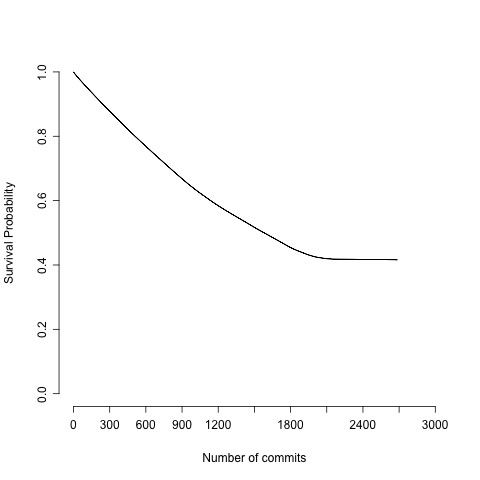
\epsfig{file = Bower_Commit_Scaleno-reassign_rplot.jpg, width = 4cm}}%
	}
	\subfigure[Chained Methods]{%
		{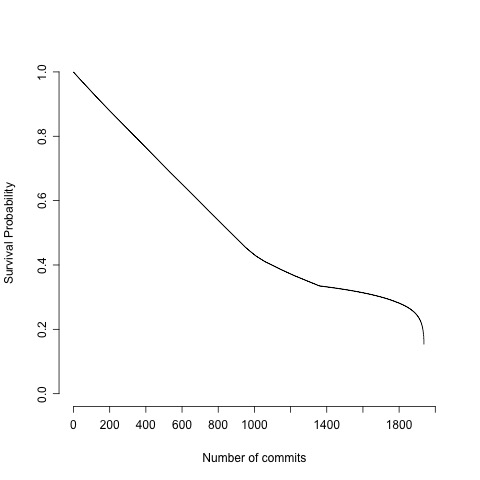
\epsfig{file = Bower_Commit_Scalecomplex-chaining_rplot.jpg, width = 4cm}}%
	}
	\subfigure[Lengthy Lines]{%
		{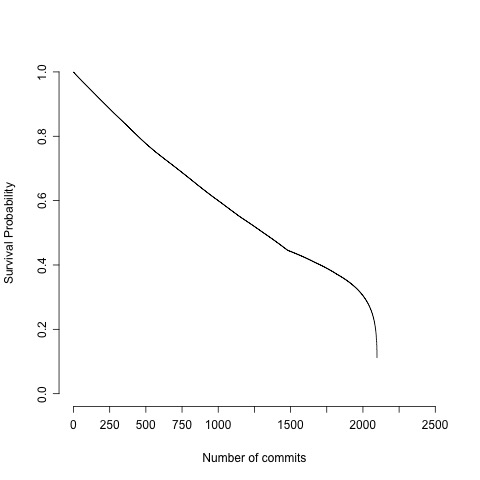
\epsfig{file = Bower_Commit_Scalemax-len_rplot.jpg, width = 4cm}}%
	}
	\subfigure[Nested Callbacks]{%
		{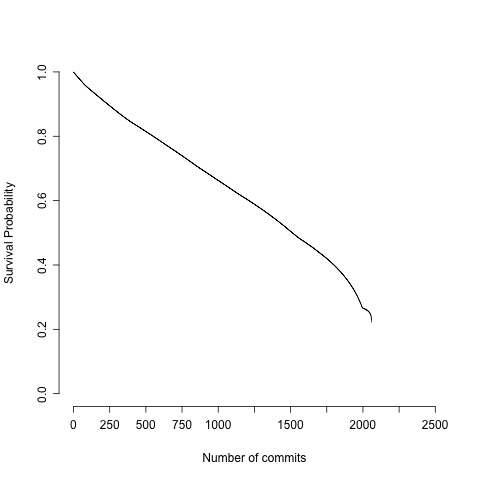
\epsfig{file = Bower_Commit_Scalemax-nested-callbacks_rplot.jpg, width = 4cm}}%
	}
	\caption{Survival analyzes of the largest smells of bower.js, with commit scale.\vspace{-10pt}}
	\label{survivalplotsbowercommitscale}
\end{figure*}

\begin{figure*}[!htbp]
	\centering%
	\subfigure[Variable Re-Assign]{%
		{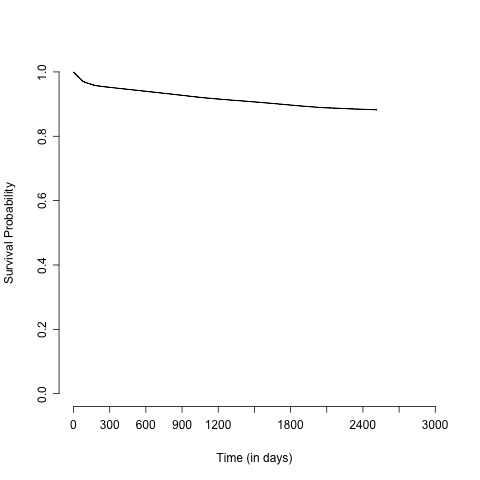
\epsfig{file = Express_no-reassign_rplot.jpg, width = 4cm}}%
	}
	\subfigure[Nested Callbacks]{%
		{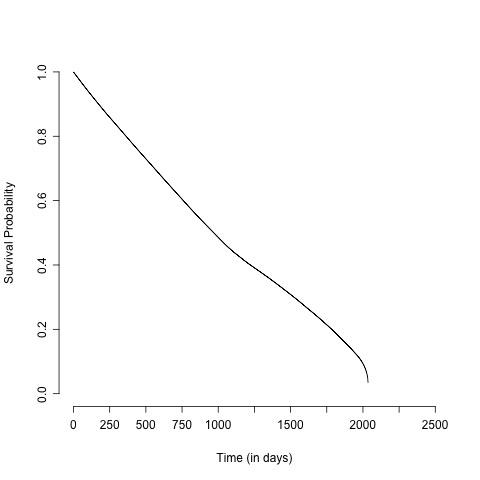
\epsfig{file = Express_max-nested-callbacks_rplot.jpg, width = 4cm}}%
	}
	\subfigure[Complex Code]{%
		{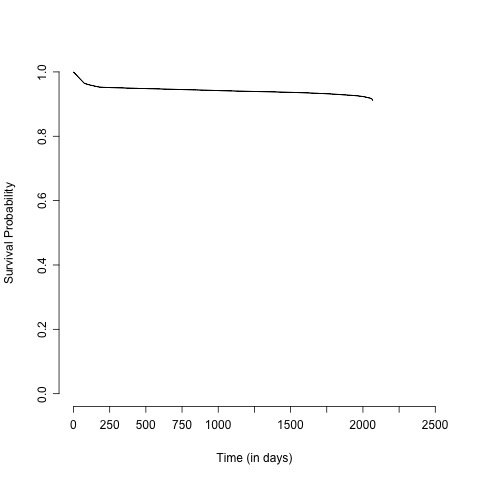
\epsfig{file = Express_complexity_rplot.jpg, width = 4cm}}%
	}
	\subfigure[Long Methods]{%
		{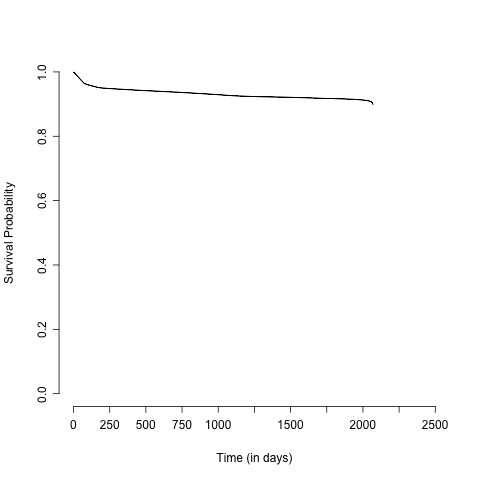
\epsfig{file = Express_max-statements_rplot.jpg, width = 4cm}}%
	}
	\caption{Survival analyzes of the largest smells of express.js.\vspace{-10pt}}
	\label{survivalplots1}
\end{figure*}

\begin{figure*}[!htbp]
	\centering%
	\subfigure[Variable Re-Assign]{%
		{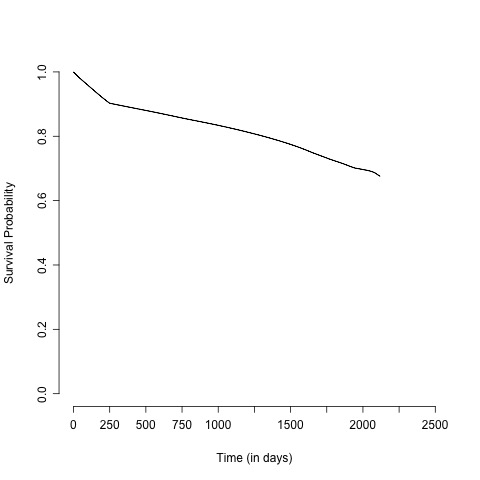
\epsfig{file = Grunt_no-reassign_rplot.jpg, width = 4cm}}%
	}
	\subfigure[Lengthy Lines]{%
		{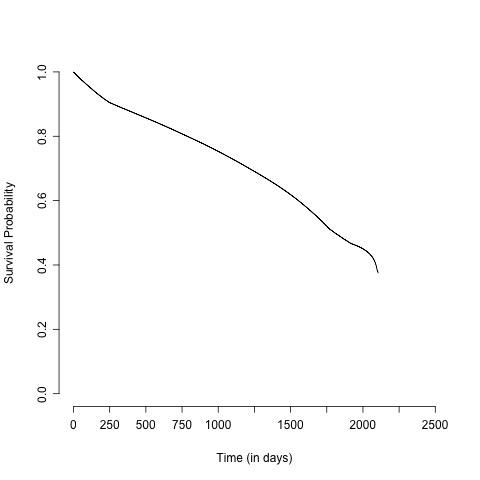
\epsfig{file = Grunt_max-len_rplot.jpg, width = 4cm}}%
	}
	\subfigure[Complex Code]{%
		{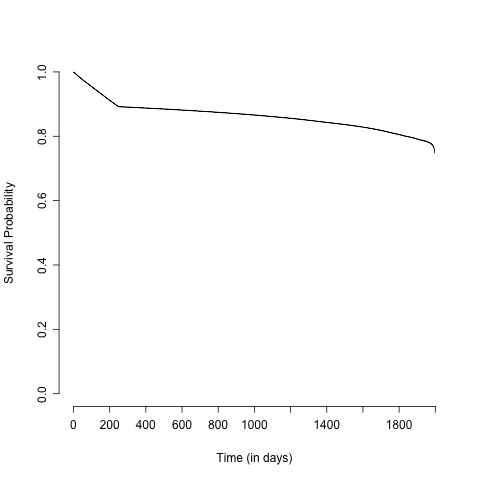
\epsfig{file = Grunt_complexity_rplot.jpg, width = 4cm}}%
	}
	\subfigure[Long Methods]{%
		{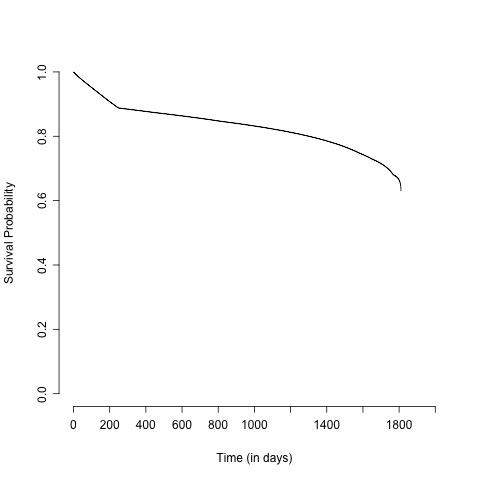
\epsfig{file = Grunt_max-statements_rplot.jpg, width = 4cm}}%
	}
	\caption{Survival analyzes of the largest smells of grunt.js.\vspace{-10pt}}
	\label{survivalplots2}
\end{figure*}

\begin{figure*}[!htbp]
	\centering%
	\subfigure[Variable Re-Assign]{%
		{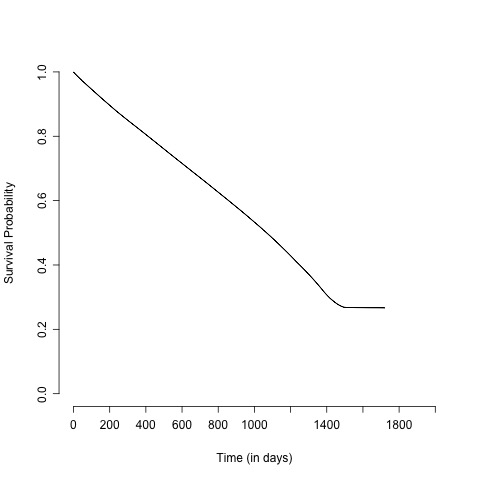
\epsfig{file = Bower_no-reassign_rplot.jpg, width = 4cm}}%
	}
	\subfigure[Chained Methods]{%
		{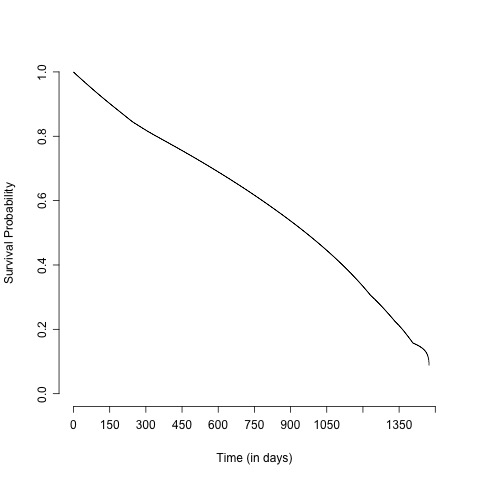
\epsfig{file = Bower_complex-chaining_rplot.jpg, width = 4cm}}%
	}
	\subfigure[Lengthy Lines]{%
		{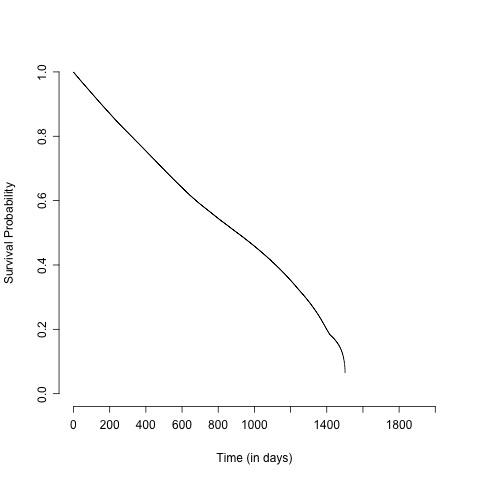
\epsfig{file = Bower_max-len_rplot.jpg, width = 4cm}}%
	}
	\subfigure[Nested Callbacks]{%
		{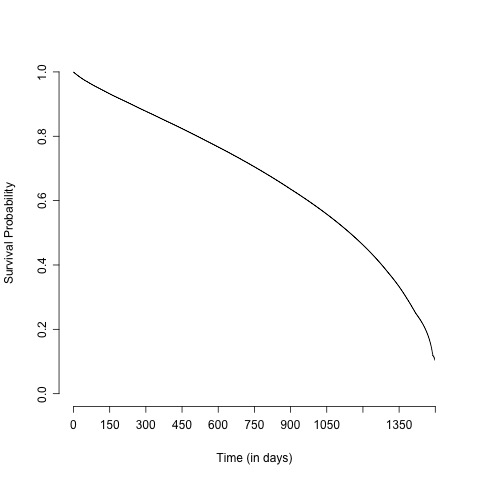
\epsfig{file = Bower_max-nested-callbacks_rplot.jpg, width = 4cm}}%
	}
	\caption{Survival analyzes of the largest smells of bower.js.\vspace{-10pt}}
	\label{survivalplots3}
\end{figure*}

\begin{figure*}[!htbp]
	\centering%
	\subfigure[Variable Re-Assign]{%
		{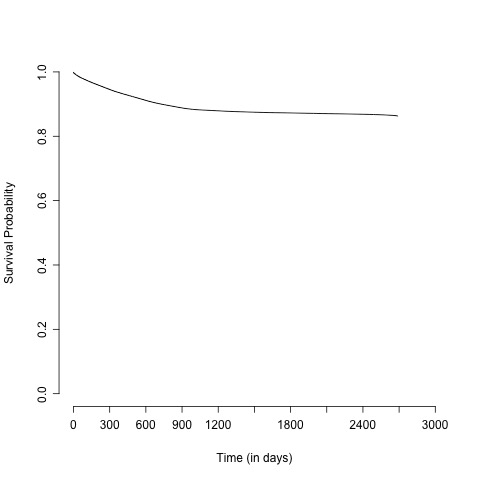
\epsfig{file = Less_no-reassign_rplot.jpg, width = 4cm}}%
	}
	\subfigure[Nested Callbacks]{%
		{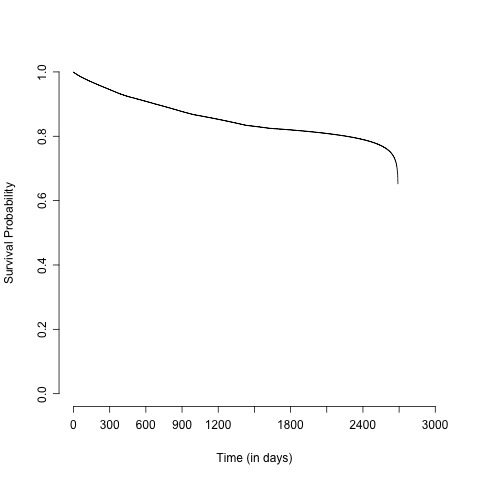
\epsfig{file = Less_max-nested-callbacks_rplot.jpg, width = 4cm}}%
	}
	\subfigure[Complex Code]{%
		{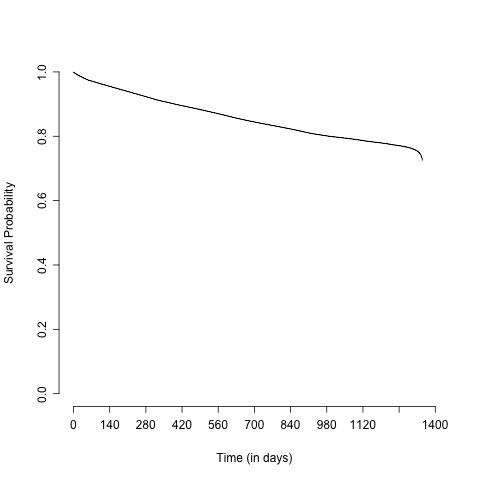
\epsfig{file = Less_complexity_rplot.jpg, width = 4cm}}%
	}
	\subfigure[Long Methods]{%
		{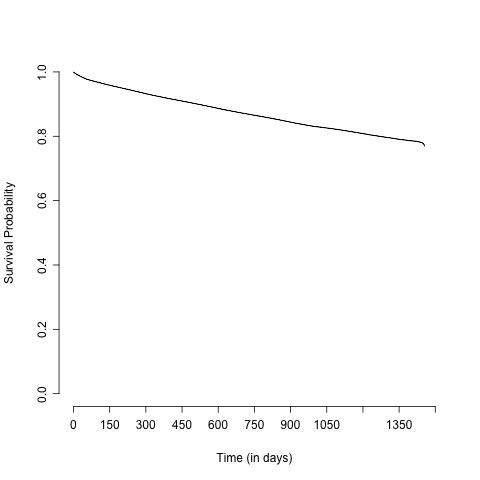
\epsfig{file = Less_max-statements_rplot.jpg, width = 4cm}}%
	}
	\caption{Survival analyzes of the largest smells of less.js.\vspace{-10pt}}
	\label{survivalplots4}
\end{figure*}

\begin{figure*}[!htbp]
	\centering%
	\subfigure[Variable Re-Assign]{%
		{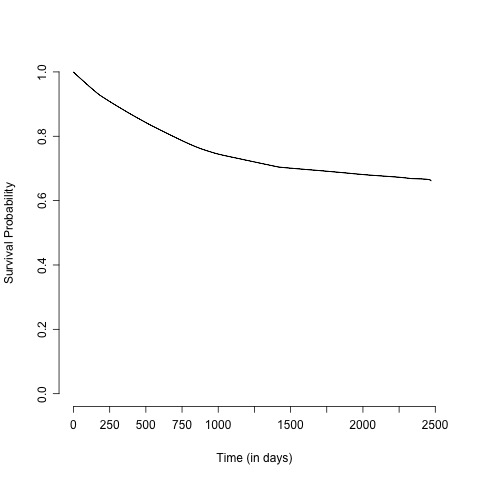
\epsfig{file = Request_no-reassign_rplot.jpg, width = 4cm}}%
	}
	\subfigure[This Assign]{%
		{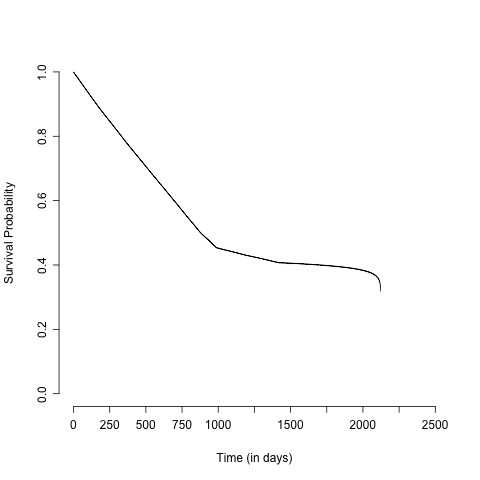
\epsfig{file = Request_this-assign_rplot.jpg, width = 4cm}}%
	}
	\subfigure[Chained Methods]{%
		{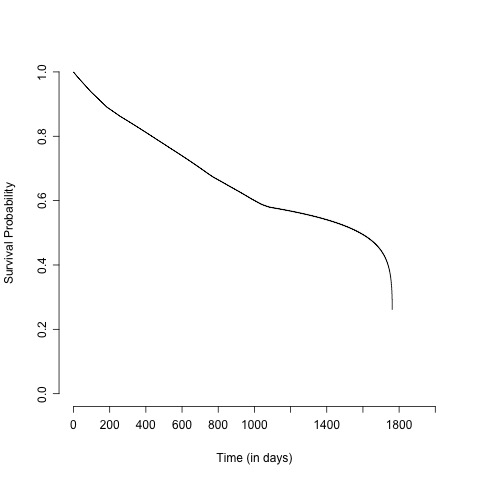
\epsfig{file = Request_complex-chaining_rplot.jpg, width = 4cm}}%
	}
	\subfigure[Nested Callbacks]{%
		{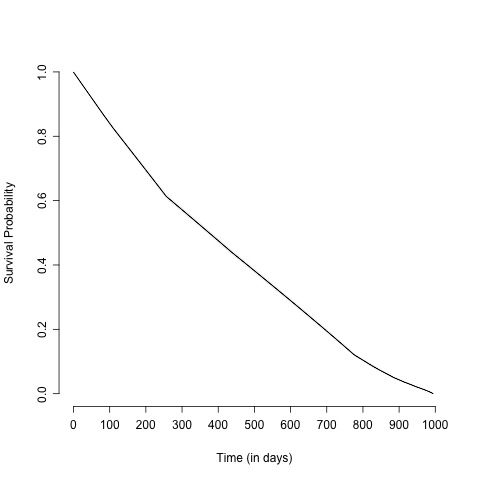
\epsfig{file = Request_max-nested-callbacks_rplot.jpg, width = 4cm}}%
	}
	\caption{Survival analyzes of the largest smells of request.js.\vspace{-10pt}}
	\label{survivalplots5}
\end{figure*}

\begin{figure*}[!htbp]
	\centering%
	\subfigure[Variable Re-Assign]{%
		{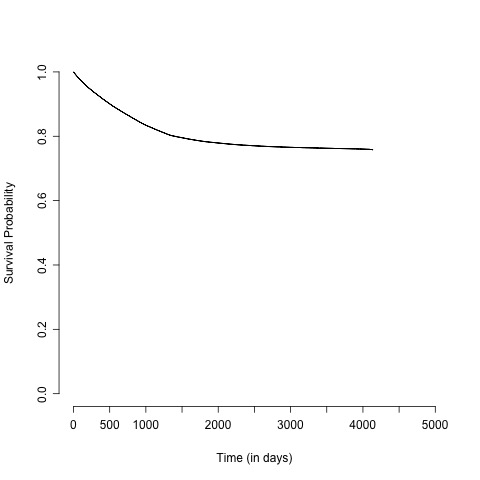
\epsfig{file = Jquery_no-reassign_rplot.jpg, width = 4cm}}%
	}
	\subfigure[Complex Switch Case]{%
		{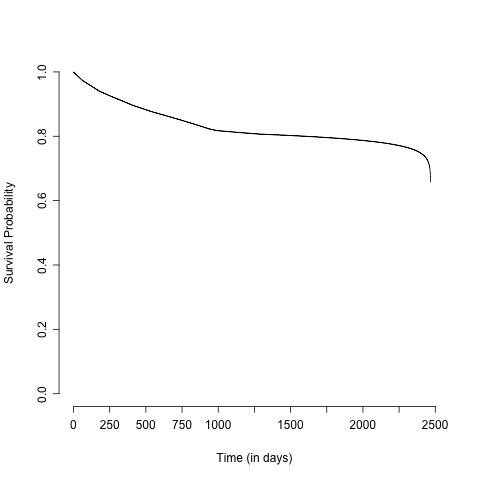
\epsfig{file = Jquery_complex-switch-case_rplot.jpg, width = 4cm}}%
	}
	\subfigure[This Assign]{%
		{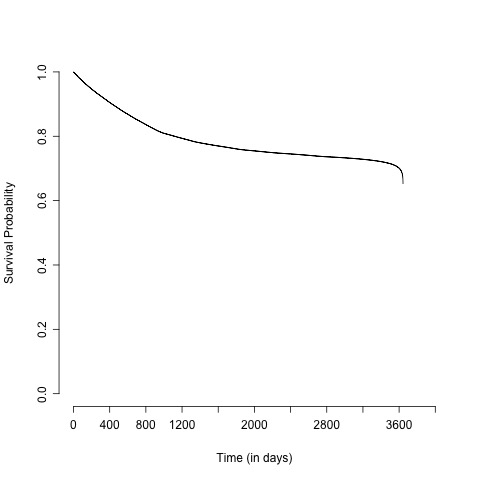
\epsfig{file = Jquery_this-assign_rplot.jpg, width = 4cm}}%
	}
	\subfigure[Chained Methods]{%
		{\epsfig{file = Jquery_complex-chaining_rplot.jpg, width = 4cm}}%
	}
	\caption{Survival analyzes of the largest smells of jquery.js.\vspace{-10pt}}
	\label{survivalplots6}
\end{figure*}

\begin{figure*}[!htbp]
	\centering%
	\subfigure[Variable Re-Assign]{%
		{\epsfig{file = Hexo_no-reassign_rplot.jpg, width = 4cm}}%
	}
	\subfigure[Lengthy Lines]{%
		{\epsfig{file = Hexo_max-len_rplot.jpg, width = 4cm}}%
	}
	\subfigure[Long Parameter List]{%
		{\epsfig{file = Hexo_max-params_rplot.jpg, width = 4cm}}%
	}
	\subfigure[Complex Code]{%
		{\epsfig{file = Hexo_complexity_rplot.jpg, width = 4cm}}%
	}
	\caption{Survival analyzes of the largest smells of hexo.js.\vspace{-10pt}}
	\label{survivalplots7}
\end{figure*}

\begin{figure*}[!htbp]
	\centering%
	\subfigure[Variable Re-Assign]{%
		{\epsfig{file = Leaflet_no-reassign_rplot.jpg, width = 4cm}}%
	}
	\subfigure[Lengthy Lines]{%
		{\epsfig{file = Leaflet_max-len_rplot.jpg, width = 4cm}}%
	}
	\subfigure[Nested Callbacks]{%
		{\epsfig{file = Leaflet_max-nested-callbacks_rplot.jpg, width = 4cm}}%
	}
	\subfigure[Long Methods]{%
		{\epsfig{file = Leaflet_max-statements_rplot.jpg, width = 4cm}}%
	}
	\caption{Survival analyzes of the largest smells of leaflet.js.\vspace{-10pt}}
	\label{survivalplots8}
\end{figure*}

\begin{figure*}[!htbp]
	\centering%
	\subfigure[Variable Re-Assign]{%
		{\epsfig{file = Ramda_no-reassign_rplot.jpg, width = 4cm}}%
	}
	\subfigure[Chained Methods]{%
		{\epsfig{file = Ramda_complex-chaining_rplot.jpg, width = 4cm}}%
	}
	\subfigure[Long Parameter List]{%
		{\epsfig{file = Ramda_max-params_rplot.jpg, width = 4cm}}%
	}
	\subfigure[Complex Code]{%
		{\epsfig{file = Ramda_complexity_rplot.jpg, width = 4cm}}%
	}
	\caption{Survival analyzes of the largest smells of ramda.js.\vspace{-10pt}}
	\label{survivalplots9}
\end{figure*}

\begin{figure*}[!htbp]
	\centering%
	\subfigure[Variable Re-Assign]{%
		{\epsfig{file = Chart_no-reassign_rplot.jpg, width = 4cm}}%
	}
	\subfigure[This Assign]{%
		{\epsfig{file = Chart_this-assign_rplot.jpg, width = 4cm}}%
	}
	\subfigure[Lengthy Lines]{%
		{\epsfig{file = Chart_max-len_rplot.jpg, width = 4cm}}%
	}
	\subfigure[Complex Switch Case]{%
		{\epsfig{file = Chart_complex-switch-case_rplot.jpg, width = 4cm}}%
	}
	\caption{Survival analyzes of the largest smells of chart.js.\vspace{-10pt}}
	\label{survivalplots10}
\end{figure*}

\begin{figure*}[!htbp]
	\centering%
	\subfigure[Variable Re-Assign]{%
		{\epsfig{file = Riot_no-reassign_rplot.jpg, width = 4cm}}%
	}
	\subfigure[Lengthy Lines]{%
		{\epsfig{file = Riot_max-len_rplot.jpg, width = 4cm}}%
	}
	\subfigure[This Assign]{%
		{\epsfig{file = Riot_this-assign_rplot.jpg, width = 4cm}}%
	}
	\subfigure[Assignment in Conditional Statement]{%
		{\epsfig{file = Riot_cond-assign_rplot.jpg, width = 4cm}}%
	}
	\caption{Survival analyzes of the largest smells of riot.js.\vspace{-10pt}}
	\label{survivalplots11}
\end{figure*}

\begin{figure*}[!htbp]
	\centering%
	\subfigure[Variable Re-Assign]{%
		{\epsfig{file = Vue_no-reassign_rplot.jpg, width = 4cm}}%
	}
	\subfigure[Lengthy Lines]{%
		{\epsfig{file = Vue_max-len_rplot.jpg, width = 4cm}}%
	}
	\subfigure[Complex Code]{%
		{\epsfig{file = Vue_complexity_rplot.jpg, width = 4cm}}%
	}
	\subfigure[Long Methods]{%
		{\epsfig{file = Vue_max-statements_rplot.jpg, width = 4cm}}%
	}
	\caption{Survival analyzes of the largest smells of vue.js.\vspace{-10pt}}
	\label{survivalplots12}
\end{figure*}

\begin{figure*}[!htbp]
	\centering%
	\subfigure[Variable Re-Assign]{%
		{\epsfig{file = Moment_no-reassign_rplot.jpg, width = 4cm}}%
	}
	\subfigure[Nested Callbacks]{%
		{\epsfig{file = Moment_max-nested-callbacks_rplot.jpg, width = 4cm}}%
	}
	\subfigure[Complex Switch Case]{%
		{\epsfig{file = Moment_complex-switch-case_rplot.jpg, width = 4cm}}%
	}
	\subfigure[Chained Methods]{%
		{\epsfig{file = Moment_complex-chaining_rplot.jpg, width = 4cm}}%
	}
	\caption{Survival analyzes of the largest smells of moment.js.\vspace{-10pt}}
	\label{survivalplots13}
\end{figure*}

\clearpage

\begin{figure*}[!htbp]
	\centering%
	\subfigure[Variable Re-Assign]{%
		{\epsfig{file = Webpack_no-reassign_rplot.jpg, width = 4cm}}%
	}
	\subfigure[Nested Callbacks]{%
		{\epsfig{file = Webpack_max-nested-callbacks_rplot.jpg, width = 4cm}}%
	}
	\subfigure[Chained Methods]{%
		{\epsfig{file = Webpack_complex-chaining_rplot.jpg, width = 4cm}}%
	}
	\subfigure[Lengthy Lines]{%
		{\epsfig{file = Webpack_max-len_rplot.jpg, width = 4cm}}%
	}
	\caption{Survival analyzes of the largest smells of webpack.js.\vspace{-10pt}}
	\label{survivalplots14}
\end{figure*}

\begin{figure*}[!htbp]
	\centering%
	\subfigure[Variable Re-Assign]{%
		{\epsfig{file = Webtorrent_no-reassign_rplot.jpg, width = 4cm}}%
	}
	\subfigure[This Assign]{%
		{\epsfig{file = Webtorrent_this-assign_rplot.jpg, width = 4cm}}%
	}
	\subfigure[Nested Callbacks]{%
		{\epsfig{file = Webtorrent_max-nested-callbacks_rplot.jpg, width = 4cm}}%
	}
	\subfigure[Chained Methods]{%
		{\epsfig{file = Webtorrent_complex-chaining_rplot.jpg, width = 4cm}}%
	}
	\caption{Survival analyzes of the largest smells of webtorrent.js.\vspace{-10pt}}
	\label{survivalplots15}
\end{figure*}

\subsection*{(RQ3) How long do code smells survive in JavaScript projects?}

\textbf{Approach}. We use the framework described in Section~\ref{extraction}, Figure~\ref{process3}, to collect information about the appearance of the 12 studied code smells in our fifteen subject systems, as well as their line localization, their content and their genealogy (which means their evolution over time from their creation to either their destruction, or the last revision of the studied system). Then, we apply the data analysis model described in Section~\ref{AnalysisRQ3} (RQ3) to our collected data. {\color{blue}As mentioned earlier, the time scale of our survival analysis is the number of days, and could have been the number of commits. Indeed, knowing how many days a smell survives in the system is more demonstrative than knowing how many commits it survives, and the number of commits scale will not bring more relevant information since the studied systems are regularly active almost everyday. Figures~\ref{survivalplots3} and~\ref{survivalplotsbowercommitscale} represent the main survival smells results for the project bower.js, respectively with number of days and commits scales, and show that both scales imply the same trend about these results. All the results with both scales appear in the Github repository of the project. For the results and the conclusions of this section, the number of days scale is used.}

\textbf{Findings}. Our results are presented in the Table~\ref{survivalsmells} for a density analysis, and in the Figures~\ref{survivalplots1} to~\ref{survivalplots15} for a survival analysis.
For the Table~\ref{survivalsmells}, for each system and each smell, the third column corresponds to the number of killed smells (\ie{} smells that have been removed), and the fourth to the number of survived smells. The sum of both columns gives us the number of created smells. The fifth column reports, in percentage, the proportion of smells created at the files birthdate, relatively to the number of created smells. In order to not overload the presentation of our results, we only report the descriptive statistics for the four most relevant smells, which means those for which the number of created is the most considerable. Finally, Table~\ref{survivalsmells} reports, for each studied system, general statistics (\textsl{SUM} lines), computed by summing the statistics of the twelve studied smells.
For the Figures~\ref{survivalplots1} to~\ref{survivalplots15}, we plot the survival analysis for each studied system, and for each smells reported in the Table~\ref{survivalsmells}, still in order to not overload the presentation of our results. The $Y$-axis corresponds to the chance of surviving of a given smell type, $x$ days after its introduction into the code base.\\
The results presented in Table~\ref{survivalsmells} show that smells are not often introduced during files evolution and changes, but rather at the creation of files. Indeed, when we look at the \textsl{SUM} lines, from 34.5\% (for \textsl{leaflet}) to 91.4\% (for \textsl{less}) of the smells are introduced at the file birthdate, meaning that developers should pay attention to the quality of their code when they create a JavaScript file, because it is precisely at this moment that most of the smells are introduced into the system. We also notice that, for the major part of the studied systems (eight out of fifteen), more than 20\% of the smells created still survive presently; and for thirteen systems, more than 10\% of the smells created are now present in these systems. It reveals that a significant part of the smells are never removed from the system once they are introduced in the code. Plus, after analyzing the commits of the studied systems, it is interesting to notice that most of the time, the killed smells are removed at the same time as the file containing them (and not because of a refactoring). \\
Table~\ref{survivalsmells} gives us also an overview of the smells lifetime, and we observe that for most of the systems (nine out of fifteen), the median and average days of survival of the most significant smell types are greater than $100$ days; and for fourteen systems out of fifteen (except \textsl{hexo}), at least one of the most sizable smell types has an average and median lifetime greater than $100$ days. This observation highlights that in general, smells tend to survive a very long time inside the system once they are introduced. Finally, Table~\ref{survivalsmells} also presents an interesting result, which is that the smell \textsl{Variable Re-assign} is always the most considerable smell type (in our fifteen studied systems) in term of number of created smells, and its survival rate follows the trend of the sum of the smells (when we consider all the smells created in the system). For every studied system, over $1000$ \textsl{Variable Re-assign} smells are created, and for eight systems out of fifteen, the number of created smells of this type exceeds $10000$. Once again, \textsl{Variable Re-assign} is at the heart of our analysis, because as said previously, it is one of the most risky smell in terms of fault-proneness.\\
According to Figures~\ref{survivalplots1} to~\ref{survivalplots15}, the four most significant smell types of each studied system have a considerable chance of surviving $500$ days after their introduction. This is indeed the case for all the most significant smell types for nine systems out of fifteen (except \textsl{request}, \textsl{chart}, \textsl{moment}, \textsl{webtorrent}, and \textsl{vue}), with over $50$\% chance of surviving $500$ days after the introduction of their largest smell types. Also, for fourteen studied systems out of fifteen (except \textsl{vue}), at least one of the most sizable smell types has more than $50$\% chance of surviving $500$ days after its smells introduction. Plus, for twelve systems out of fifteen (except \textsl{bower}, \textsl{vue}, and \textsl{webtorrent}), the \textsl{Variable Re-assign} smell type has more than $50$\% chance of surviving $1500$ days after its introduction. These observations show the trend of the smells of the studied systems to be persistent and survive a long time after their introduction in the code, and also the significance of \textsl{Variable Re-assign}, which is strongly linked to fault-proneness, and is the most proliferated smell type in the studied systems, with a very high chance of surviving over time.

\hypobox{Most of the studied smells (from 34.5\% to 91.4\%) are introduced during the creation of JavaScript files. Once introduced, in most of the systems (eight systems), more than 20\% of the studied smells are not removed and have a high chance of surviving a very long time. Plus, \textsl{Variable Re-assign}, which is the most fault-prone smell is also the smell with the highest chance of surviving over time.}

{\color{blue}Even if JavaScript is highly dynamic and allows reassign variables, we show here that re-assign smells are bad practices widely used, rarely removed from the projects, and more likely to introduce faults in systems. This observation is not so much surprising, as reassign statements make the code particularly unreadable, especially when they are widely present in a same portion of code. Hence, developers need to pay attention when they introduce reassign variables. They should consider refactoring their code to remove re-assign smells regularly.}

%}

\section{Threats to validity}\label{threats}

In this section, we discuss the threats to validity of our study following common guidelines for empirical studies~\cite{robert2002case}.

\textbf{Construct validity threats} concern the relation between theory and observation. In our study, threats to the construct validity are mainly due to measurement errors. %Our metrics in our survival analysis might not reflect all characteristics related to defects \Foutse{do you mean code smells or faults?} and we could include more metrics specifically related to source code or even the review process of fault fixes. \Foutse{you should explain why your results are still valid regardless of this limitation!} %We leave the selection of more metrics as a future work.
The number of previous faults in each source code file was calculated by identifying the files that were committed in a fault fixing revision. This technique is not without flaws. We identified fault fixing commits by mining the logs searching for certain keywords (\ie{} ``fix",``\#", and ``gh-") and certain bug IDs, as explained in Section~\ref{extraction}. Following this approach, we are not able to detect fault fixing revisions if the committer either misspelled the keywords, or failed to include any commit message, or includes in a non common way the bug IDs. Nevertheless, this heuristic was successfully used in multiple previous studies in software engineering~\cite{jaafar2013mining,shihab2013studying}. The SZZ heuristic used to identify fault-inducing commits is not 100\% accurate. However, it has been successfully used in multiple previous studies from the literature, with satisfying results. In our implementation, we remove all fault-inducing commit candidates that only changed blank or comment lines, {\color{blue} and all of those that were too far from the issue date. We followed all the recommendations proposed by Da Costa et al.~\cite{da2017framework} to improve the accuracy of the SZZ heuristic.  Also, as explained in Section~\ref{extraction}, we only analysed commits from the master branch of each project. Even if all the other branches information are represented in the master branch, the time introduction of bugs and smells can be different. However, the issue of time difference between master branch introduction and other branches introduction of the studied smells or bugs concerns a few data of our extraction.} When tracking smells over time during the construction of the genealogies of the smells, we set a similarity threshold of 70\%, meaning that if two smells of the same type have a similarity greater than 70\%, they are considered to be the same. Obviously, this threshold is not perfect and can associate two different smells together, or dissociate two smells, which are in reality the same. However, we performed a sensitivity analysis, with threshold values at 70\%,  80\% and 90\% and obtained similar results. %   it in order to see if some significant differences would appear, but no relevant difference was revealed.
	
%When analyzing the \emph{smelliness} of files that experienced fault-inducing changes, we only tracked the presence of the smell in the file as a whole. Hence, the smell contained in the file may not have been involved in the changed lines that induced the fault. %we assume the a smell didn't get touched if it is removed from a section of a file and another added to another section of the same file in the same commit.}

\textbf{Internal validity threats} concern our selection of systems and tools. % other possible explanations for some of our observations. We used SZZ algorithm to find original commits that induced bugs later in the project. The SZZ algorithm is a an heuristic approach and might not contain all 100\% true positive original commits.
The metric extraction tool used in this paper is based on the AST provided by ESLint. The results of the study are therefore dependent on the accuracy of ESLint. However, we are rather assured that this tool functions properly as it is being used widely by big companies. \eg{} Facebook, Paypal, Airbnb.
%The threshold selected to find smelly codes is by top 10\%  ... The different numbers for threshold might change the category of files as smelly or not smelly. Hence, different strategies to define a threshold may lead different results at the end.
We chose a logarithmic link function for some of our covariates in the survival analysis. It is possible that a different link function would be a better choice for these covariates. However, the non-proportionality test implies that the models were a good fit for the data. %We leave the selection of different link functions for each covariate as future work.
Also, we do not claim causation in this work, we simply report observations and correlations and tries to explain these findings.

\textbf{Threats to conclusion validity} address the relationship between the treatment and the outcome. We are careful to acknowledge the assumptions of each statistical test.

\textbf{Threats to external validity} concern the possibility to generalize our results. In this paper, we have studied fifteen large JavaScript projects. We have also limited our study to open-source projects. Still, these projects represent different domains and various project sizes. Table~\ref{studiedsystems} shows a summary of the studied systems, their domain and their size. Nevertheless, further validation on a larger set of JavaScript systems, considering more types of code smells is desirable. %done to further validate our results. %\New{We have limited this study to a list of 12 types of code smells; however, the list includes the most common bad practices in JavaScript. Future works should also consider other types of code smells.}

\textbf{Threats to reliability validity} concern the possibly of replicating our study. In this paper, we provide all the details needed to replicate our study. All our fifteen subject systems are publicly available for study. The data and scripts used in this study is also publicly available on Github\footnote{\url{https://github.com/DavidJohannesWall/smells_project}}.
%Therefore, we can not generalize 100\% our results to other JavaScript projects particularly closed-source ones. Even though our study includes a small subset of available JavaScript software, we attempted to mitigate this issues by selecting a diverse number of projects.

%{\color{blue}


\section{Related Work}\label{sec:related}
In this section, we discuss the related literature on code smell and JavaScript systems.
Code Smells~\cite{fowler1997refactoring} are poor design and implementation choices that are reported to negatively impact the quality of software systems. They are opposite to design patterns~\cite{Gam95} which are good solutions to recurrent design problems.
%Other researches have been done on Javascript before. Most of the previous studies on Javascript have been done on client side security of Javascript applications. Saxena \ea developed a system to explore the execution space of client side Javascript applications to find security vulnerabilities \cite{saxena2010symbolic}. On the other study, they proposed a dynamic analysis technique to discover validation vulnerabilities in client side Javascript applications systematically \cite{saxena2010flax}. Richards \ea studied the dynamic behavior of Javascript by performing an empirical study on how and why the dynamic features of Javascript are being used \cite{richards2010analysis}. Bielova conducted a survey on Javascript security policies for client side applications and proposed a detailed comparision of the runtime monitoring based security technique for Javascript applications \cite{bielova2013survey}. Tripp and Weisman presented a hybrid-analysis solution to automate the assessment of Javascript client side application by combining white-box and black-box methodologies \cite{tripp2011hybrid}. Hallaraker \ea also proposed an approach based on monitoring Javascript code execution to detect malicious code behavior \cite{hallaraker2005detecting}.
The literature related to code smells generally falls into three categories: (1) the detection of code smells~(e.g.,~\cite{Khomh11-BGB,fard2013jsnose}); (2) the evolution of code smells in software systems (e.g.,~\cite{chatzigeorgiou2010investigating,CodeSmells_overtime,peters2012evaluating,tufano2015and}) and their impact on software quality (e.g., ~\cite{shatnawi2006investigation,khomh2012exploratory,Abbes11,jaafar2013mining,tufano2015and,d2010impact,palomba2018diffuseness});
and (3) the relationship between code smells and software development activities (e.g.,~\cite{Sjoberg13QEC,Abbes11}).  
Our work in this paper, falls into the second category. We aim to understand how code smells affect the fault-proneness of JavaScript systems. Li and Shatnawi~\cite{shatnawi2006investigation} who investigated the relationships between code smells and the occurrence of errors in the code of three different versions of Eclipse reported that code smells are positively associated with higher error probability. In the same line of study, Khomh et al.~\cite{khomh2012exploratory} investigated the relationship between code smells and the change- and fault-proneness of 54 releases of four popular Java open source systems (ArgoUML, Eclipse, Mylyn and Rhino). They observed that classes with code smells tend to be more change- and fault-prone than other classes. Tufano et al. \cite{tufano2015and} investigated the evolution of code smells in 200 open source Java systems from Android, Apache, and Eclipse ecosystems and found that code smells are often introduced in the code at the beginning of the projects, by both newcomers and experienced developers. Sjoberg et al.~\cite{Sjoberg13QEC}, who investigated the relationship between code smells and maintenance effort reported that code smells have a limited impact on maintenance effort. However, Abbes et al.~\cite{Abbes11} found that code smells can have a negative impact on code understandability. Recently, Fard et al. \cite{fard2013jsnose} have proposed a technique named JNOSE to detect 13 different types of code smells in JavaScript systems. The proposed technique combines static and dynamic analysis. They applied JNOSE on 11 client-web applications and found ``lazy object" and ``long method/function" to be the most frequent code smells in the systems. WebScent~\cite{nguyen2012detection} is another tool that can detect client-side smells. It identifies mixing of HTML, CSS, and JavaScript, duplicate code in JavaScript, and HTML syntax errors. ESLint \cite{ESLint}, JSLint \cite{JslinT} and JSHint \cite{JSHint} are rule based static code analysis tools that can validate source codes against a set of best coding practices. Despite this interest in JavaScript code smells and the growing popularity of JavaScript systems, to the best of our knowledge, there is no study that examined the effect of code smells on the fault-proneness of JavaScript server-side projects. This paper aims to fill this gap. {\color{blue}To remove code smells in software systems, developers often rely on refactorings, which are behavior preserving code transformations. Gatrell and al.~\cite{gatrell2015effect} explain how refactoring can be help improve the quality of software systems and reduce fault-proneness. } %of software.}

%These previous studies raised the awareness of the community about the potential negative impact of code smells on the quality of object oriented systems and recommended that developers apply refactorings to remove code smells from their systems. %of y recommend applying refactoring to remove such interactions of anti-patterns.

%Jaafar et al.~\cite{jaafar2013mining} examined the fault-proneness of classes sharing a static or a co-change relationship with a class containing a code smell and reported hat  an empirical study to analyze anti-patterns dependencies in more than 165000 commits of three Java open source software (ArgoUML, JFreeChart, and XerecesJ). They showed that, classes that have static relationship as well as the classes that have co-change relationship with anti-patterns are more likely to be fault-prone than others.

%and smelliness happens as a consequence of evolution and maintenance activities which can even be introduced by refactoring operations.  al.~\cite{Khomh:2012:ESI:2158916.2158921} show that there is a relation between antipatterns and the bug-proneness of a file. These studies provide empirical evidences on the relation between antipatterns and bugs.
%Khomh et al. \cite{khomh2012exploratory} who investigated the relationship between the presence of code smells and software change- and fault-proneness
%Tufano et al. \cite{tufano2015and} studied a large change history of 200 open source projects in Java (Android, Apache and Eclipse) and found that code smells can be formed since the beginning of a project by both newcomers and experienced deveopers and smelliness happens as a consequence of evolution and maintenance activities which can even be introduced by refactoring operations. Khomh et al. \cite{khomh2012exploratory} investigated the relationship between the presence of anti-patterns and software change- and fault-proneness on 54 releases of four popular Java open source systems (ArgoUML, Eclipse, Mylyn and Rhino). They discovered that classes with code smells tend to be more change-and fault-prone than the other classes. Jaafar et al. \cite{jaafar2013mining} conducted an empirical study to analyze anti-patterns dependencies in more than 165000 commits of three Java open source software (ArgoUML, JFreeChart, and XerecesJ). They showed that, classes that have static relationship as well as the classes that have co-change relationship with anti-patterns are more likely to be fault-prone than others.

%On the other hand, less studies aimed the quality and maintainability of Javascript applications \cite{nguyen2012detection}.
%A number of efforts have been done on tools that assist developers to better maintain their web applications. JSLint \cite{JslinT} is a static code analysis tool that can validate source codes against a set of best code practices. In a more closely related work, Fard et al. \cite{fard2013jsnose} proposed a technique that combines static with dynamic analysis to detect 13 different types of code smells. They applied their JNOSE on 11 web applications an found that ``lazy object" and ``long method/function" are amongst the most frequent code smells. WebScent ~\cite{nguyen2012detection} detects client-side smells and basically identifies mixing of HTML, CSS, and JavaScript, duplicate code in JavaScript, and HTML syntax error.
%
%However, non of mentioned works have examined the effect of code smells on a very important aspect of software, i.e., fault-proneness in JavaScript projects.

%Gizas \ea compared the latest release of 7 popular client side Javascript libraries and reported their overall quality, performance and validity \cite{gizas2012comparative}. Those studies however are only focused on the client side Javascript application.
%In this paper, we analyzed the quality of server side JavaScript applications and conduct an empirical study on five popular server side JavaScript frameworks over 537 releases to explore the survival of smelly codes in terms of catching software bugs.

%In the following sections we introduce the concept of NodeJS and NPM and discuss why this platform needs more attention in the researchers' community.

%\subsection*{JavaScript and Nodejs}
%\mytitle{JavaScript and Nodejs} JavaScript is a powerful, flexible and popular scripting programming language. It is the most commonly used programming language on both front-end and back-end with more than 90\% usage on the front-end and more than 54\% on the back-end \cite{so:survay2016}. It also has the most active repositories and total pushes on Github \cite{githut}.
%\Foutse{The systems investigated in this paper use NodeJS and NPM?} \Foutse{we need to explain why it is important to know these two concepts otherwise we should remove them...right now its not clear to me if they are useful for understanding the work presented in the paper, Amir please exlain.....}
%\mytitle{Nodejs} (also called Node) is an open source platform to run JavaScript on the server side. The core is based on Google's JavaScript runtime engine called V8. Node and V8 are mostly written in C and C++. Although V8 mainly supports running client-side JavaScript codes, Node uses its power to support long-running, real-time, scalable and memory efficient server-side network applications \cite{tilkov2010node}. Node is also famous for its event-driven nature and non-blocking I/O model, which makes it a perfect fit for data-intensive and network applications. On the first quarter of 2015, Joyent, IBM, Microsoft, PayPal, Fidelity, SAP and The Linux Foundation joined forces to bring neutral and open governance support to the Node community \cite{nodeFoundation}. The growing popularity of JavaScript raises the demand for good design practices and style-guides.

%\subsection*{NPM}
%\mytitle{NPM} Nodejs comes with its own package manager called NPM (Node Package Manager). NPM enables developers to install community libraries and their dependencies easily through the command-line interface \cite{tilkov2010node}. By the time of writing this paper, there are more than 310,000 distinct modules registered on NPM. With average growth rate of more than 400 modules per day, it is the most popular registry on the web \cite{modulecounts}. This shows how the popularity of using community libraries are increasing. NPm has increased the usage of community libraries drastically, thanks to its simple and easy to use APIs. % of NPM increased the usage of using community libraries drastically.
%Developers can add third-party modules as dependency of their application using simple commands. But, this raises the questions about the quality and security of those modules. In March 2016, a developer removed all of his modules from NPM. One of the modules called \texttt{left-pad}\footnote{https://www.npmjs.com/package/left-pad} had been used by thousands of other modules living in NPM. The removal of this small module with only 11 lines of code, broke thousands of other modules \cite{reg2016lp, med2016lp}. This event was a strong illustration of the impact that community modules can have on JavaScript applications. %is indicates how the security and quality of community modules impact JavaScript applications.




\section{Conclusion}\label{conclusion}

%In this paper, we developed an extension for ESLint in order to extract a set of code smells from five JavaScript projects. Then, we use Cox hazard models to find out whether smelly codes are harmful, and what specific types of code smells make it more defect-prone. We analyze the models to understand which covariates play significant roles in determining defects. We used log-rank test to measure whether a significant statistical difference exists between survival probabilities of smelly codes and non-smelly codes. We also demonstrate the validity and accuracy of our models using the non-proportionality assumption test. Moreover, we designed a survey to have JavaScript practitioners' opinions on the different types of source code practices, i.e., source codes with smells against source codes with the same rationale but without smells.
In this study, we examine the impact of code smells on the fault-proneness of JavaScript systems. We also examine the survival of code smells in JavaScript systems. Regarding fault-proneness, we compare the time until a fault occurrence in JavaScript files that contain code smells and files without code smells, tracking faults and smells at the line level {\color{blue}of each file, in order to ensure that the considered faults affected smelly code lines.}  %refine the correlations between faulty and smelly lines}. %at the li, {\color{blue}with two different approaches: line grain, and line grain including dependencies approaches}. {\color{blue}This quantitative study also present some descriptive statistics about the twelve studied smells, as well as their survival by computing their lifetime.}
Results show that JavaScript files without code smells have hazard rates at least 33\% lower than JavaScript files with code smells. %{\color{blue}, using our line grain analysis}. 
In other terms, the survival of JavaScript files against the occurrence of faults increases with time if the files do not contain code smells. We further investigated hazard rates associated with different types of code smells and found that ``Variable Re-assign", ``Assignment in Conditional Statements", and ``Complex Code" smells have the highest hazard rates. Regarding the survival of code smells in the systems, results show that code smells are generally introduced in the JavaScript files when the files are created. ``Variable Re-assign" which occur frequently in JavaScript systems can survive for a very long time in a system. JavaScript developers should consider removing \emph{Variable Re-assign} code smells from their systems in priority since this code smell is consistently associated with a high risk of fault. They should also prioritize \emph{Assignment in Conditional Statements}, \emph{Complex Code}, \emph{This Assign}, \emph{Nested Callbacks}, and \emph{Long Parameter List} code smells for refactoring.

%
%  the occurenand a qualitative study by posting a survey among more than 1000 JavaScript developers, we have made two findings. First, we found that smelly code is more risky than non-smelly code; the risk seems to be system independent. We discovered that on average non-smelly codes have hazard rates 65\% lower than smelly codes. In other terms, the survival of all files against defects increases with time if they do not hold code smells. Second, in our findings we observed that all code smells do not equally affect software maintainability and reliability since variable-reassign (\textsl{var.reassign}) and assignment in condition (\textsl{cond.assign}) code smells have higher hazard rate in comparison to the other types of smells identified by our Cox model and survey.


%\textbf{Future work.}

%conference papers do not normally have an appendix

% use section* for acknowledgment
%\section*{Acknowledgment}
%The authors would like to thank... \cite{latexcompanion}

% trigger a \newpage just before the given reference
% number - used to balance the columns on the last page
% adjust value as needed - may need to be readjusted if
% the document is modified later
%\IEEEtriggeratref{8}
% The "triggered" command can be changed if desired:
%\IEEEtriggercmd{\enlargethispage{-5in}}

% references section

% can use a bibliography generated by BibTeX as a .bbl file
% BibTeX documentation can be easily obtained at:
% http://mirror.ctan.org/biblio/bibtex/contrib/doc/
% The IEEEtran BibTeX style support page is at:
% http://www.michaelshell.org/tex/ieeetran/bibtex/
%\bibliographystyle{IEEEtran}
% argument is your BibTeX string definitions and bibliography database(s)
%\bibliography{IEEEabrv,../bib/paper}
%
% <OR> manually copy in the resultant .bbl file
% set second argument of \begin to the number of references
% (used to reserve space for the reference number labels box)
%\begin{thebibliography}{1}

%\bibitem{IEEEhowto:kopka}
%H.~Kopka and P.~W. Daly, \emph{A Guide to \LaTeX}, 3rd~ed.\hskip 1em plus
%  0.5em minus 0.4em\relax Harlow, England: Addison-Wesley, 1999.

%\end{thebibliography}
\balance
\bibliographystyle{IEEEtran}
\bibliography{references}

% that's all folks
\end{document} 